% -----
% -- Introduction
% --
\chapter{Introduction}
\vspace{-2em}

\section{Prelude}

I am thinking of a data structure for managing collections of objects. It provides O(1) insert and update operations. It has native hardware support on all modern platforms. It has a long history of use. It's proven, and it's lightning fast.

Unfortunately, support for it in my favourite language, Haskell~\cite{haskell98-report}, appears to be somewhat lacking. There are people that would tell me that it's not needed~\cite{peyton-jones:ifp}, that there are other options~\cite{okasaki:pure-data}, that it's bad for parallelism~\cite{cann:retire-fortran} and bad for computer science in general~\cite{backus:liberate}. They say that without it, programs are easier to understand and reason about. Yet, it seems that every time I start to write a program I find myself wanting for it. It's called \emph{the~store}.

The \emph{mutable} store, that is. I want for real destructive update in a real functional language (for my own, particular,  subjective definition of `real'). I wanted it for long enough that I decided I should take a PhD position and spend the next several  years of my life trying to get it. 

Soon after starting I came to realise two things:
\begin{enumerate}[1)]
\item That the problem was real, and that many people were aware of it.
\item That this was \emph{not} a new problem.
\end{enumerate}

\clearpage{}
\section{The Problem}
Functional programming is many things to many people, but at the heart of it is one central idea. Programs should be expressed in terms of higher order functions, referred to as \emph{combining forms} in Backus's seminal paper \cite{backus:liberate}, instead of as imperative sequences of commands which update a global store.

The folklore promises that as functional programs admit more algebraic laws than their imperative counterparts, they will be easier to express and reason about. It also promises that functional programs have the potential to run faster, with the imagined speedup being partly due to freedom from the `von Neumann bottleneck', that is sequential access to the global store, and partly due to optimising transforms which can be carried out due to the algebraic laws \cite{santos:compilation}. 

After 30 years of intense research, several industry strength compilers \cite{peyton-jones:compilation-by-transformation, nocker:clean, tofte:mlkit-4.3.0, macqueen:sml}, and countless research papers, both of these promises have been delivered on --- yet curiously, functional languages have not replaced imperative ones in mainstream software engineering.

There are a myriad of endlessly debated reasons for this apparent lack of use, and most will be quite familiar to the people likely to be reading this thesis. Often touted candidates include organisational inertia and marketing pressure exerted by large corporations seeking to cement their own particular language into the psyche of the industry programmer \cite{gosling:java-standard}. It is no doubt easy to form these opinions, especially if one is a researcher or academic in the field of programming languages. Almost by definition, we spend the majority of our time working with our own systems and attending conferences where the presentations are given by people in similar circumstances.

In recent years this situation has been recognised by the functional programming community itself, hence the creation of forums that seek to collect reports of industry experience with its languages \cite{wadler:cufp}. The conclusion of many of these presentations simply reiterates what we have known all along --- that functional programming is wonderful and the application of higher order functions, pattern matching and strong typing (for some) leads to shorter development times and more reliable software.

By all accounts the community is thriving and much software is being written, yet the majority of it continues to be from graduate students and researchers in the field of programming language theory. Of this fact one can easily be convinced by visiting an arbitrary web-based job placement agency and comparing search results for ``Haskell'' or ``O'Caml'' versus any one of ``Java'', ``Perl'', ``Ruby'', ``C++'' or ``Python''.

Are Haskell and O'Caml destined to be The Velvet Underground of programming languages, where hardly anyone has heard them, but everyone who does forms a band?\footnote{After a quote attributed to Brian Eno. The Velvet Underground were a rock music group active in the late 60's, early 70's. They were highly influential, yet initially unsuccessful in a commercial sense.}

\subsubsection{Something's missing?}
What if we were to take a step back from the glory of functional programming, and instead focus on what might be missing? After all, if functional languages could do everything that imperative languages could, \emph{as well} as having strong typing, pattern matching, higher order functions and associated goodness, then at least there would be no \emph{technically} based reason not to use them.

With this in mind, this thesis takes the position that an important missing feature from all current functional languages is real destructive update. A programmer should be free to update an arbitrary data structure in their program, with minimal runtime overhead, and with minimal interference from the type system or language design. 

Note the use of the word ``interference''. In one sense, a language is a structure for formulating and communicating ideas, but in another it is a barrier to a true expression of intent. In an imperative language the programmer can update their data when and where they see fit, whereas in a typical functional language, they cannot. We seek to remove this barrier.

This work is embodied in the Disciplined Disciple Compiler (DDC)\footnote{When dealing with a field that separates languages into ``pure'' and ``impure'', the religious connotations are already present. We make no apologies for the name.}. ``Disciple'' being the name of the language it compiles, and ``Disciplined'' invoking the type and effect discipline \cite{talpin:discipline} of Talpin and Jouvelot which forms the basis of our type system. Wherever possible, we have avoided creating yet another functional language (YAFL) that no-one is likely to use. Disciple's syntax is based on Haskell, and DDC itself is written in Haskell. This allows us to leverage a huge body of existing people, ideas and code.
Keeping the source and implementation languages similar will also make it easy to bootstrap DDC in future work.

As destructive update is the source of all our problems, we start with a discussion of \emph{why} it should be included in a language in the first place. Having convinced ourselves that it is really needed, we will examine how it is supported in existing functional languages, and argue that this support is inadequate. We will discuss the notion of purity and how it benefits a language. We will also consider what it means for a language supporting destructive update and other side effects to be pure, and whether the formal notion of purity is useful in practice. Disciple allows arbitrary structures to be updated, and functions to have arbitrary side effects. Instead of relying on state monads, we use a type based analysis to recover mutability, effect and data sharing information from the program being compiled. We use an intermediate language similar to System-Fc~\cite{sulzmann:system-Fc} and our analysis recovers enough information to do the same code transformation style optimisations as a highly optimising compiler such as GHC~\cite{peyton-jones:compilation-by-transformation}. We will discuss some of the practical problems with using lazy evaluation as the default method, and why space leaks are so common in lazy programs. Disciple uses strict evaluation by default, but allows the programmer to introduce laziness when desired. We use the type system to ensure that the combination of destructive update and laziness does not change the meaning of the program compared with the strict case.

This chapter outlines our approach and the reasons we have chosen it. Chapter 2 discusses the type system in detail, and Chapter 3 outlines the inference algorithm. Chapter 4 describes our core language and gives a proof of soundness for its type system. Chapter 5 summarises what we have learned so far and suggests avenues for future work.






% --------------------
\section{Why destructive update matters}
\label{intro:update}

Destructive update is the process of changing the value of an object in-place, by overwriting and hence destroying its old value. Without destructive update we cannot change the values of existing objects, only allocate new ones. 

With deference to Turing completeness, destructive update is \emph{simply not required} to write programs. Likewise, almost every feature of a particular language can be shown to be superfluous. Tiny systems such as the Lambda Calculus, Conway's game of life, and the Rule 30 cellular automata are Turing complete~\cite{rendell:life, cook:universal}, and hence capable of universal computation. On the other hand, no one writes programs in them, at least not directly.

When considering language features we must always start from a practical, and therefore subjective viewpoint. When we say ``destructive update matters", we mean that a large enough subset of programmers find it useful that it warrants consideration by all.

We suggest that destructive update furnishes the programmer with two important and powerful tools, and that these tools are either too cumbersome or too inefficient to create without it. The first tool is a set of efficient array-like data structures for managing collections of objects, and the second is the ability to broadcast a new value to all parts of a program with minimal burden on the programmer.


% --------------------
\subsection{Efficient data structures require destructive update}
For a mechanical device such as an internal combustion engine, efficiency is defined as the ratio of useful work output to the amount of energy input to the device~\cite{giancoli:efficiency}. For a \emph{computational} device such as a collection structure, we could reasonably define its efficiency as being the number of insert and update operations that can be completed per hardware clock cycle. 

We pay no attention to the difficulty of designing the structure in the first place. Like internal combustion engines, the development of common data structures is best left to teams of experts, permitting the end user to focus on their own specific tasks.

When the number of objects to be managed is known beforehand, the simplest collection structure is the array. In a typical garbage collected runtime system, the allocation of an array requires just three machine instructions. We test the top-of-heap pointer to ensure enough space is available, write the object header word, and then advance the pointer. The update of a particular value is also straightforward. Suppose we have three registers: R1 holding a pointer to the array, R2 holding the new value, and R3 holding the index of the value to be updated. Many processors can perform this update with just one or two instructions~\cite{sun:sparc-assembly, intel:instruction-set}.

\begin{center}
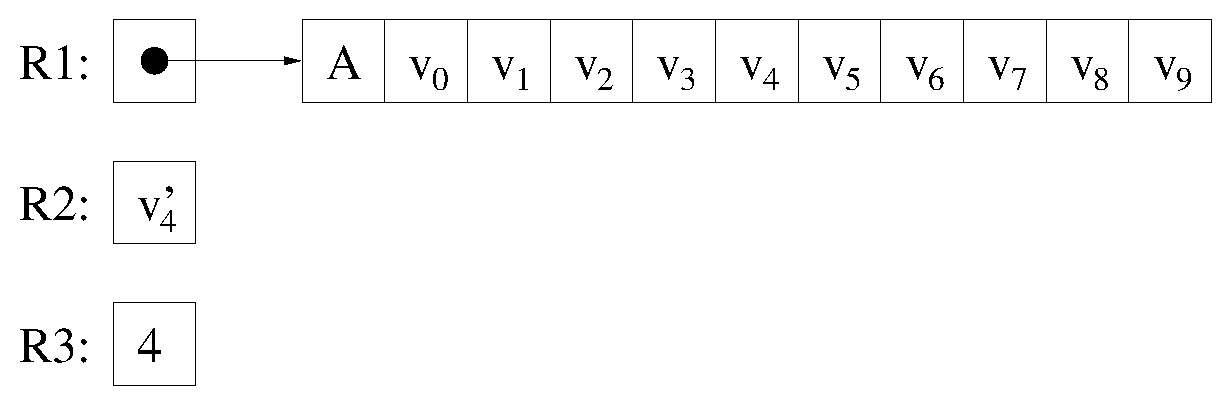
\includegraphics[scale=0.5]{1-Introduction/fig/destructive/data-array10}
\end{center}

Of course, due to pipelining and cache effects, the number of machine instructions executed for an operation does not relate directly to the number of clock cycles used~\cite{hennessy:computer-architecture}. However, it is a usable approximation for this discussion, and we will consider the case of updating a flat array as approaching 100\% efficiency for array-like structures.

Perfect efficiency would be achieved if every update operation completed in the minimum number of clock cycles possible on the available hardware. For most applications, perfect efficiency is unlikely to ever be achieved by a statically compiled program, as it is too difficult to accurately simulate pipeline states and data hazards in a multi-tasking system. 

Ignoring cache effects, the efficiency of an array is independent of how many elements it containts. It costs no more to update a value in a 1000 element array than to update one in a 10 element array.


% --------------------
\subsubsection{Functional arrays are unacceptably slow}
Without destructive update we cannot change an array object once it is allocated, but we can side-step this problem by creating a new object instead of updating the old one. A simple method is to allocate a whole new array and copy the old values into it, with the new value in place of the one that is being updated. This works, but is a disaster for performance. Assuming we need one machine instruction for each value copied, performing an update on a 10 element array now requires 10 instructions, plus three to do the allocation. This represents a miserable 7.7\% efficiency compared with a single instruction destructive update. For a 1000 element array we need at least 1003 instructions, representing approximately 0.1\% efficiency. This is clearly unacceptable.


% --------------------
\subsubsection{Tree structures are only a partial solution}
We can recover some of this ground by using a tree structure instead of a flat array. If we store values in the internal nodes of a balanced binary tree then we need $n$ nodes for $n$ values, and the tree is $\text{ceil} (\log_2(n))$ levels deep. Unfortunately, to change a value in the tree we must still allocate a new node. As this new node will be at a different address from the old one, we must then rebuild all of its parents so that the tree references the new node instead of the old one. For example, in the tree on the next page, to update $v_7$ we must reallocate the node that contains it as well as the nodes of $v_6$, $v_8$ and $v_5$.

\begin{center}
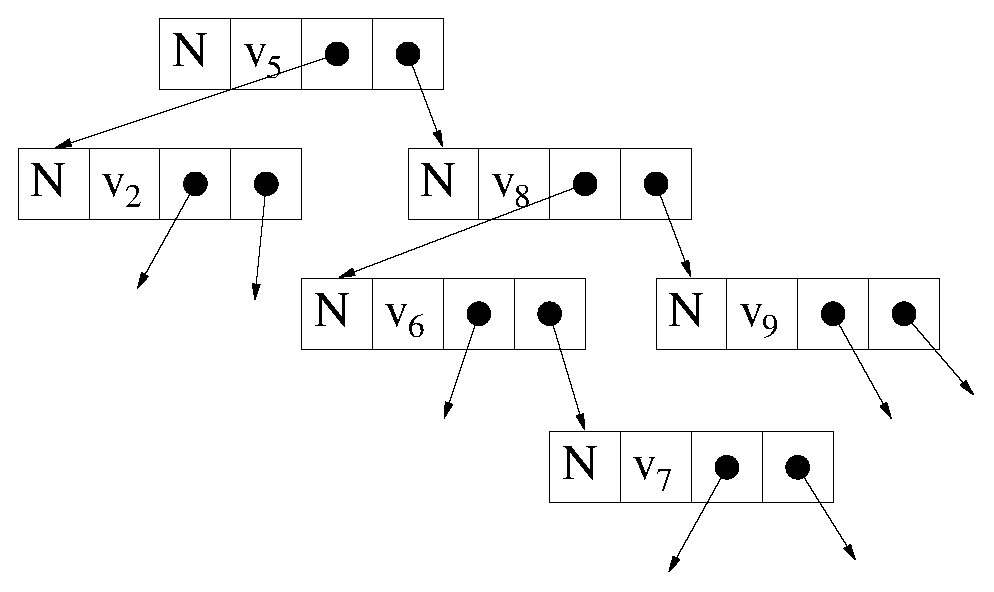
\includegraphics[scale=0.5]{1-Introduction/fig/destructive/data-tree}
\end{center}

For a small number of values, using a binary tree is \emph{worse} than copying the whole array for each update, because each node contains an object header and two pointers instead of just a value. A balanced tree of 1000 elements is 10 levels deep, and as a rough approximation, half of the nodes lie at the bottom of the tree. If we were to update one of these nodes then we would need to reallocate all of its parents, which equates to 9 * 4 = 36 words of space. Not all nodes are at this level, but we haven't accounted for finding the node to be updated in the first place either. For a back-of-envelope calculation we could expect an average of at least 50 machine instructions to be required to update a node in this tree. This equates to 2\% efficiency when compared with destructive array update of a similarly sized array.

Another option is to use trees of a higher order, perhaps a quadtree or a B-tree structure like the one shown in the following diagram. Adding more values per node reduces the depth of the tree. It also reduces the number of nodes we must rebuild when performing an update, but at the cost of making each node larger. 

\begin{center}
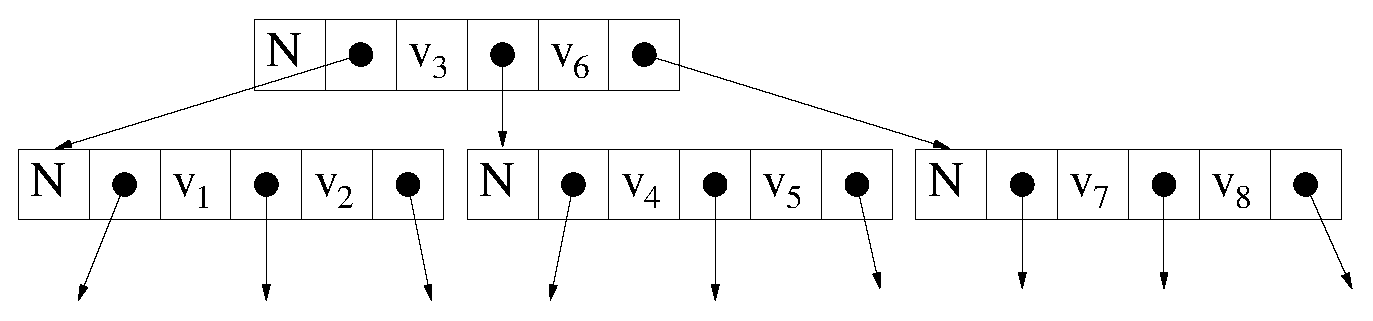
\includegraphics[scale=0.5]{1-Introduction/fig/destructive/data-btree}
\end{center}

For a full (2,3)-tree with two keys and three branches per node, each node is 6 words long including the object header. Every extra level provides three times the number of nodes present in the previous level, and for 1000 values we need a little more than 6 levels. If we say that each node to be updated has an average of 5 parent nodes, this equates to 5 * 6 = 30 words of space to be reinitialised when updating a node. This isn't much better than the previous case.

Many algorithms naturally use an array as their primary collection structure. If, for the lack of destructive update, we are forced to a tree instead, then we automatically impose a $\log(n)$ slowdown on our algorithm's run time. To access an element in a tree we must traverse its structure, but array access can be performed in constant time. This slowdown is in addition to a substantial constant factor due to the extra book-keeping data that must be maintained, such as object headers and branch pointers that are not needed when using arrays. In \cite{ponder:inefficient} Ponder gives a list of algorithms for which no equivalent, array-less algorithm of similar complexity is known. 


% --------------------
\subsubsection{The limit}
There are an infinite variety of possible structures for simulating arrays, and trees represent just a few. By this stage, an astute reader may be thinking about all their own favourite structures and how much better they are than the ones outlined here \cite{okasaki:pure-data, okasaki:intmaps}. As we are talking about machine instructions and constant factors, not just algorithmic complexity, there are also a huge variety of low level details to consider. Details include instruction selection, caching, data layout, pointer compression \cite{lattner:pointer-compression}, and using ``diff arrays'' which rely on destructive update behind the scenes for efficiency, whilst presenting a functionally pure interface. An example of pointer compression is to replace each of the pointers in an object by offsets from a base pointer, instead of including the store address in full. This can result in substantial space savings for pointer heavy programs on 64 bit machines, where the size of a particular data structure is only a tiny fraction of the available address space. Diff arrays use a destructively updateable array for the current state of the structure, and updates to the structure are implemented by physically updating this array. Old states of the array are represented by a list of differences to apply to the current state, so old states become slower and slower to access as the program progresses.

There are many avenues for improvement, but without destructive update we are still hamstrung by the need to allocate objects to represent new program states. Consider a maximally efficient structure which requires only a single, tiny object to be allocated for each update. At the least, we could expect this new object to contain a header word, the new value, and a pointer to the rest of the structure: 

\begin{center}
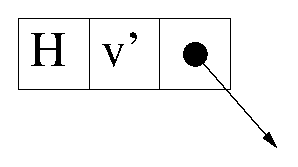
\includegraphics[scale=0.5]{1-Introduction/fig/destructive/data-tiny}
\end{center}

\vspace{-1em}
However, the allocation and initialisation of this object will still require at least five machine instructions, three for allocation and two to write the new value and pointer. For some applications a constant five-fold slow down is of no consequence, but for others it is a deal breaker. 


\clearpage{}
% --------------------
\subsubsection{Tuples and records are also arrays}

At the machine level, tuples and record objects are often very similar to arrays. We can implement records by representing each field as a pointer to the object containing its value, so at this level the record is simply an array of pointers. A record object with 5 fields would contain a header word and five pointers. Consider then the following record type from DDC:

\begin{lstlisting}
data SquidS 
    = SquidS
    { stateTrace           :: Maybe Handle			
    , stateTraceIndent     :: Int
    , stateErrors          :: [Error]
    , stateStop            :: Bool 
    , stateArgs            :: Set Arg	
    , stateSigmaTable      :: Map Var Var
    , stateVsBoundTopLevel :: Set Var
    , stateVarGen          :: Map NameSpace VarBind 
    , stateVarSub          :: Map Var  Var 
    , stateGraph           :: Graph
    , stateDefs            :: Map Var Type
    , statePath            :: [CBind]
    , stateContains        :: Map CBind (Set CBind)
    , stateInstantiates	   :: Map CBind (Set CBind)
    , stateGenSusp         :: Set Var
    , stateGenDone         :: Set Var
    , stateInst            :: Map Var (InstanceInfo Var Type)			
    , stateQuantifiedVars  :: Map Var (Kind, Maybe Type)
    , stateDataFields      :: Map Var ([Var], [(Var, Type)]) 
    , stateProject         :: Map Var (Type, Map Var Var)	
    , stateProjectResolve  :: Map Var Var
    , stateClassInst       :: Map Var [Fetter] }
\end{lstlisting}

This record represents the state of our type inferencer while it is reducing constraints. The meaning of the fields is not important for this discussion. We include this data type to make the point that real records can contain upwards of 22 separate fields. No matter how efficiently the internal sets, maps and graphs are implemented, without destructive update we cannot change the value of a field without rebuilding at least part of the record object. If we must rebuild it all, then this is at least 22 times slower than using destructive update.

In a language without destructive update we must allocate and initialize new objects to represent new program states. This a drastically less efficient alternative. In practice, even if a language does not support the destructive update of arbitrary structures, attempts are made to introduce it in a more restricted form. In \cite{sastry:order-of-evaluation-analysis} Sastry presents an analysis to determine an order of evaluation for array access and update operations, that allows the updates to be implemented destructively. Besides being first order only, the trouble with many such analyses is that when they fail to introduce an update at an important point in the program, the programmer is left with little recourse to add it manually. There is also the problem of determining which updates \emph{should} have been implemented destructively, but weren't. 

As discussed in \S\ref{intro:monads}, Haskell includes a monadic sub-language that supports the destructive update of select structures such as arrays. However, this sub-language introduces its own problems, and algebraic data such as records and lists cannot be similarly updated. In \cite{sansom:time-profiling} Sansom describes the time profile of an early version of GHC, and mentions that the use of a monadic mutable array over an association list improved the performance of type substitution by a factor of 10. When combined with other improvements, this resulted in a 20x speedup of the type checker as a whole.
 
If a particular programmer does not use functional arrays or large records in their programs, then they may not be aware of the run-time cost of using them. However, those who do are looking down the barrel of a five fold slow-down, or worse, compared with other languages.


% --------------------
\subsection{Destructive update helps to broadcast new values}
\label{Intro:Update:broadcast}
There is an often rehearsed argument that the expressiveness of a language is more important than efficiency, because improvements to processor speed will quickly recover any lost ground. The standard counter is to say that the common man wants their new and faster computers to do \emph{new and faster things}, not the original things less efficiently.

These arguments can also be applied to destructive update. ``Surely'', the antagonist offers, ``a five fold slow-down is not \emph{that} bad. Moore's law says we'll have that back in four years, and look at all the extra compiler optimisations we can do now that the language is pure!''.

Computational efficiency may or may not matter to a particular programmer, but the level of abstraction offered by the language should matter to all. We will now move away from concerns over run time speed, and instead focus on the expressiveness of the language itself. Consider a set of program modules which all reference a single, shared value. This value could be a cursor position or timing value, something that changes often and is of interest to many separate modules. We will refer to this value as X. In a language with destructive update we can place X in a container structure and have each module access it via a pointer:

\begin{center}
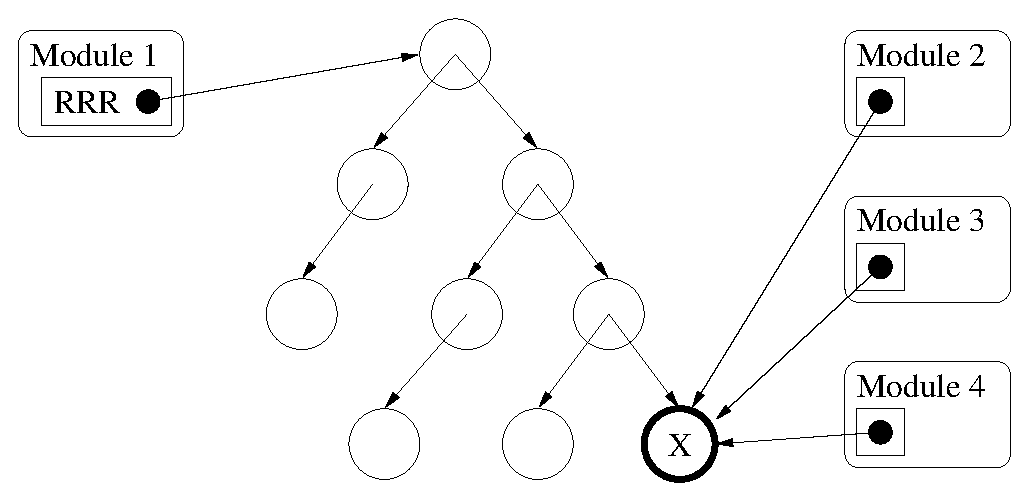
\includegraphics[scale=0.6]{1-Introduction/fig/destructive/broadcast-direct}
\end{center}

Using destructive update, one module can modify X and the new version is immediately visible to others. Notice that module 1 has a reference to the top of the container structure as well as a description of how to find the value of interest. In this example the container is a binary tree and the value is accessable by following three right branches from the root node. On the other side, modules 2, 3, and 4 do not need to know how to locate X within its container because they have a pointer directly to it. This second group of modules is not interested in the container or any other value contained within.

Without destructive update, a module cannot change X directly, nor can it change the pointers within client modules so that they reference any new objects it might create. The programmer is forced to rewrite all modules so that they reference the top level of the container structure, and include a description of how to find the value of interest.

\begin{center}
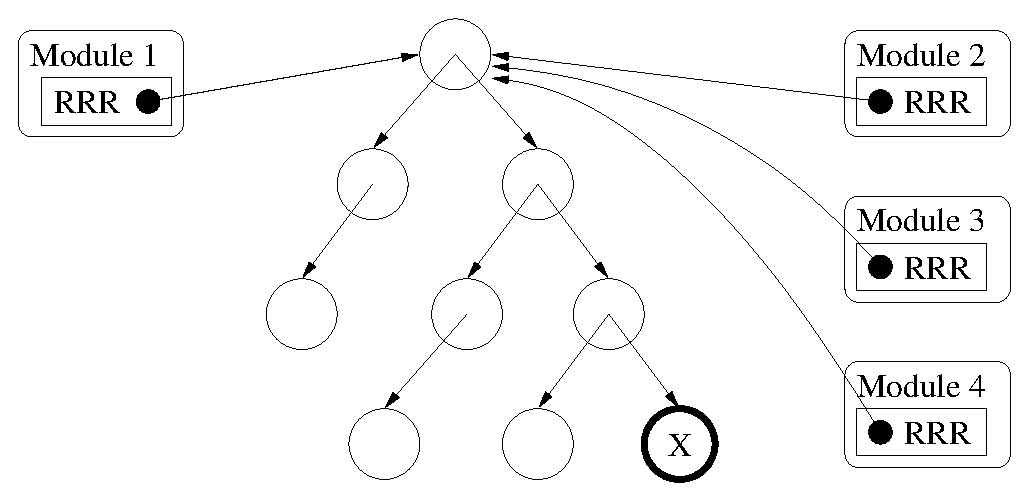
\includegraphics[scale=0.6]{1-Introduction/fig/destructive/broadcast-toplevel}
\end{center}

By doing this we have reduced the level of abstraction in the program. Whereas modules 2, 3, and 4 are only interested in the value X, they must now also concern themselves with the container structure and how to find and update elements contained within.

This problem is compounded when a shared value is logically part of several containers. Perhaps X is also present in a graph structure, and the tree is used to represent a set of objects which must be written to disk when the program finishes. The modules that wish to update the shared value must have knowledge of all structures which contain it.

Shared values like the one described here are often needed to write interactive programs such as Frag \cite{cheong:frag}. In Haskell, variables holding timing values, mouse positions and other user interface states are typically bundled up into a record of IORefs. This in turn requires all code which accesses these values to be written in the IO monad, a point we will return to in \S\ref{intro:monads}.


% --------------------
\subsubsection{Updating nested records in Haskell is painful}

Haskell 98 has an conspicuously poor record system. In itself this is not a new observation, but we pause to discuss it because we feel the problem arises in part from the lack of destructive update in the ambient language. Standard complaints include the records not being light weight, not being extensible, and that all field names are in the top level scope \cite{peyton-jones:records}. In addition, we consider the syntax for updating nested records to be unusable.
 
The following code defines three record types with two fields each. Type \texttt{R1} contains type \texttt{R2}, and type \texttt{R2} contains type \texttt{R3}. Notice the prefixes \texttt{r1}, \texttt{r2} and \texttt{r3} on each field name. In Haskell, field names pollute the top level name space, so we can't have a field named \texttt{field1} in \texttt{R1} as well as in \texttt{R2} without creating a name clash.

\clearpage{}
\begin{lstlisting}
data R1 = R1 { r1Field1  :: Int
             , r1Field2  :: R2 }

data R2 = R2 { r2Field1  :: Char
             , r2Field2  :: R3 }

data R3 = R3 { r3Field1  :: Bool
             , r3Count   :: Int }
\end{lstlisting}

We will create a record value of type \texttt{R1} as an example. Similarly to the previous section, we treat the field \texttt{r3Count} as a shared value that many program modules will be interested in. When the record is created we will initialise this field to zero. The exact values used for the other fields are not important for this example.

\begin{lstlisting}
record1 = R1 { r1Field1 = 5
             , r1Field2 = 
                  R2 { r2Field1 = 'a'
                     , r2Field2 =
                          R3 { r3Field1 = False
                             , r3Count  = 0 }}}
\end{lstlisting}

Extracting the counter field from the structure is straightforward. Each field name becomes a projection function which takes the record and produces the field value, for example \texttt{r1Field1 :: R1 -> Int}. We can make use of the function composition operator to extract the count field using a pleasing syntax:

\begin{lstlisting}
count  = (r3Count . r2Field2 . r1Field2) record1
\end{lstlisting}

Updating the counter is another matter entirely. As we do not wish to modify the other fields in the structure, we must unpack and repack each level in turn. This process corresponds to reallocating parents when updating a node in a tree. Unfortunately, this time we cannot write a cute recursive function to do so because the records at each level have different types. The following diagram shows the structure of the nested records:

\begin{center}
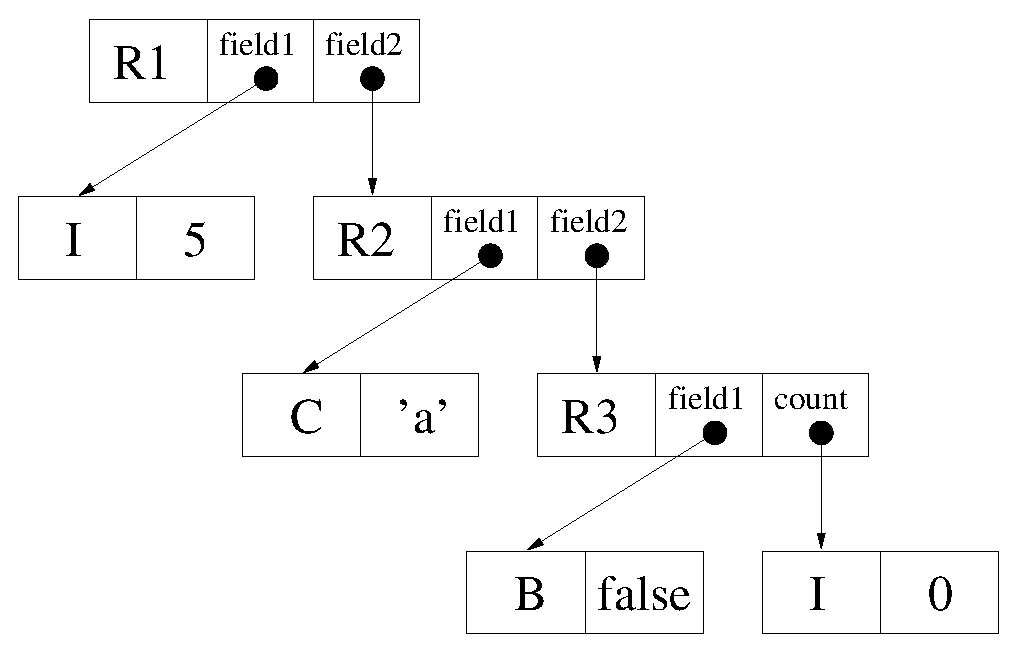
\includegraphics[scale=0.5]{1-Introduction/fig/destructive/broadcast-record}
\end{center}

\clearpage{}
\begin{center}
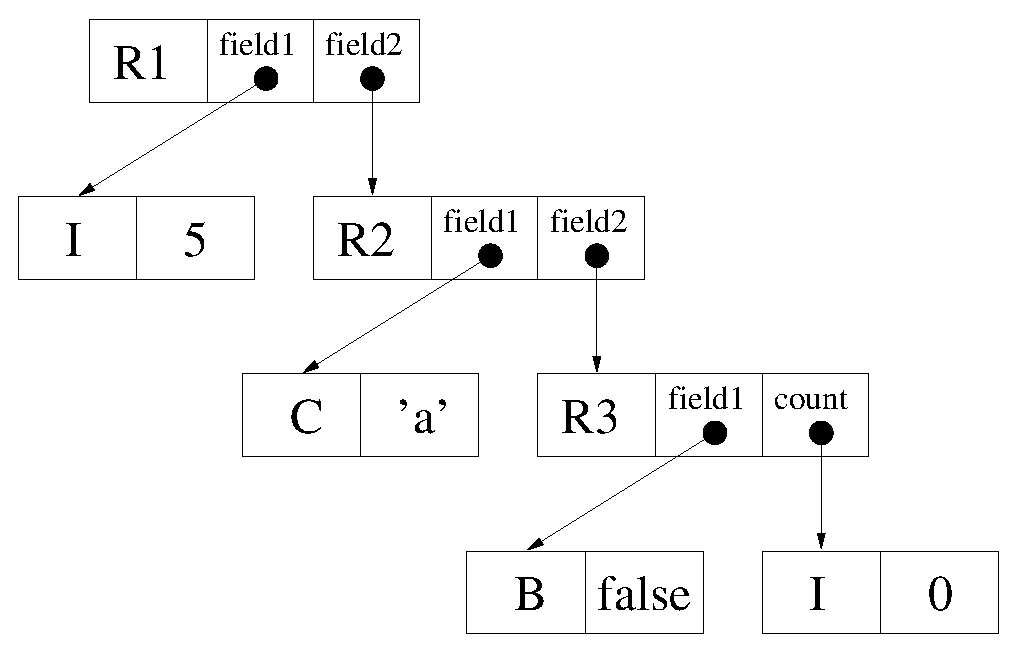
\includegraphics[scale=0.5]{1-Introduction/fig/destructive/broadcast-record}
\end{center}

If we wish to change the \emph{count} field in this structure to the value 1, we must allocate a new object containing this value. We must then rebuild the \texttt{R3}, \texttt{R2} and \texttt{R1} nodes so that the structure references this new object while retaining the pointers to the other nodes. Here is the gory Haskell expression:

\begin{lstlisting}
record2
  = record1 { r1Field2 = 
      (r1Field2 record1) { r2Field2 = 
         ((r2Field2 . r1Field2) record1) { r3Count = 1 }}}
\end{lstlisting}

Clearly this is not something a typical programmer would enjoy writing. The field names and the variable \texttt{record1} are repeated twice each, the line must be broken into fragments to fit on the page, it does not indent well, and there is much visual noise.

It is worse when we need to update this field with a non-trivial expression. Consider the simple act of incrementing \texttt{r3Count}. We can use layout to reduce the noise, but it is still quite bad:
\begin{lstlisting}
record3
  = record2 { 
      r1Field2 = (r1Field2 record2) {
      r2Field2 = ((r2Field2 . r1Field2) record2) {
      r3Count  = (r3Count . r2Field2 . r1Field2) record2 + 1 
    }}}
\end{lstlisting}
The need to write such tedious code to perform such a simple update would be a deal breaker for many programmers.\footnote{It certainly is for the author.}

Consider an equivalent statement in an imperative language, such as C++.
\begin{lstlisting}
record2.field2.field2.count += 1
\end{lstlisting}
Destructive update allows the programmer to focus solely on the element of interest, while leaving the others untouched. Granted, the above statement does not have the same semantics as the Haskell version because it modifies the original object instead creating a new one. If this behaviour is required then many imperative, object oriented languages support a fragment such as:
\begin{lstlisting}
record3 = record2.copy()
record3.field2.field2.count += 1
\end{lstlisting}
To the surrounding program these two simple statements have the same effect as the Haskell expression shown above, with the added advantage that the concepts of \emph{copy} and \emph{update} are clearly separated.

In C++ we can make life even easier for the programmer. We can create a reference to the field of interest and increment it without any knowledge of the surrounding record structure:
\begin{lstlisting}
int* countRef = &(record.field2.field2.count)

(*countRef) += 1;
\end{lstlisting}

Admittedly, references and destructive update can be used for evil as well as for good. Many confusing programs can be constructed in which different program modules communicate via shared mutable objects in a way which is entirely non-obvious to the casual observer, and almost impossible to debug. The counter to this argument is to say that confusing programs can be written in any language, and a good carpenter can hammer a nail into a wall without smashing their own fingers.

We should note that the problem of updating nested records in Haskell can be made easier by generic programming libraries such as `Scrap Your Boilerplate'~\cite{lammel:scrap-your-boilerplate} (SYB) and DriFT~\cite{hinze:generic-programming-in-haskell}. Although these systems can help, we feel they are not complete solutions as they lack the efficiency and ease of use of destructive update. SYB style systems tend to traverse uninteresting parts of a structure when performing an update, resulting in a significant performance penalty~\cite{mitchell:neil}. DriFT is a preprocessor which can automatically generate update functions for each of the fields in a record, though it does not support nested update as per the previous example. When implementing DDC we defined tuples of get and set functions for each field, along with combinators to compose these functions and to update fields deep within nested records. We have found this to be a serviceable yet tedious approach, as we have not yet written a preprocessor to generate the tuples. This approach also does not solve the problem of field names being in top level scope.


\clearpage{}
\section{What is purity?}
\label{intro:purity}

Although the word \emph{purity} has many varied meanings, most would agree that the following expression is pure:

\code{
	$(\lambda x. \idouble x) \ (\isucc 5)$
}

To reduce this expression call-by-value, we first evaluate the argument and then substitute into the body of the function.

\code{	
	$(\lambda x. \idouble x) \ (\isucc 5)$ \\
	$\eto (\lambda x. \idouble x) \ 6$ \\
	$\eto \idouble \ 6$ \\
	$\eto 12$
}
 
When we reduce the same expression call-by-name, we substitute the argument first, yielding the same result.

\code{
	$(\lambda x. \idouble x) \ (\isucc \ 5)$ \\
	$\eto \idouble \ (\isucc \ 5)$ \\
	$\eto \idouble \ 6$ \\
	$\eto 12$
}

In the simply typed lambda calculus, the order in which function applications are evaluated does not affect the end result. This behavior is also known as the Church-Rosser property~\cite{rosser:highlights}, or \emph{confluence}. Purity is of tremendous help to compiler writers because it gives us the freedom to reorder function applications during compilation, whilst preserving the meaning of the program. By reordering function applications we can expose many useful compiler optimisations \cite{santos:compilation}, and this well known identity of the $\imap$ function is one such example:

\code{
	$\imap \ f \ (\imap \ g \ \ixs) \ \equiv \ \imap \ (f \circ g) \ \ixs$
}

The first expression applies $g$ to each element of the list $xs$ yielding an intermediate list. It then applies $f$ to each element of this list, yielding the result. In the second expression, the composition of $f$ and $g$ is applied to each element directly, without requiring the construction of an intermediate list. As long as we are free to reorder function applications, we can optimise a arbitrary program by rewriting expressions of the first form into the second.

The Glasgow Haskell Compiler includes a myriad of similar optimisations. Simple, frequently invoked rewrites are ``baked-in'' to the compiler proper, whereas more specific identities such the one above are part of the standard libraries, or are defined by the programmer directly. The recent work on stream fusion~\cite{coutts:stream-fusion} is a prime example of library defined rewrites which depend on purity.

In contrast, the following expression is decidedly not pure:

\code{
	$\ichoose \ (\iinTrouble \ ()) \ (\ilaunchMissiles \ 5) \ (\ieatCake \ 23)$
}

The end result of this expression depends very much on the order of evaluation.  The intention is for the first argument to execute first, before choosing \emph{one} of the others. This ordering must be preserved in the compiled program, else the meaning of the program will be changed.

The concept of purity can also be applied to a language as a whole. With the Church-Rosser property in mind, Sabry defines a purely functional language to be one that satisfies the following criteria~\cite{sabry:purely}:
\begin{enumerate}
\item	it is a conservative extension of the simply typed $\lambda$-calculus.
\item	it has a well-defined call-by-value, call-by-need, and call-by-name evaluation
	functions (implementations), and
\item	all three evaluation functions (implementations) are weakly equivalent.
\end{enumerate}

We will consider the finer points of these criteria in a moment. Separate from Sabry's definition, the functional programming community generally recognises Haskell to be pure, while SML, Scheme, Fortran and C++ are said to be \emph{impure} languages. However, note that Fortran and C++ are not extensions of the $\lambda$-calculus, so are not functional either.

\subsubsection{\emph{Pure} and \emph{impure} are loaded terms}
Sabry's definition contains several subtle points, not least of which are the words being defined. The Oxford English Dictionary (OED) gives several meanings for the word ``impure''. In regards to ``a language or style'', the word has the meaning of ``containing foreign idioms or grammatical blemishes''. In this context, the ``foreign idioms'' would include interactions with the outside world such as launching missiles or eating cake. These actions are not part of the formal definition of the lambda calculus, and it is not obvious what the result will be from the function names alone. The other meaning offered by the OED is along the lines of ``not pure ceremonially; unhallowed'', or ``containing some defiling or offensive matter; dirty, unclean".

This is unfortunate terminology. In contrast, mathematical disciplines are sometimes separated into groups labeled pure and \emph{applied}. The intention is that the more pure disciplines have no immediate practical applications, but are considered worthy of study because they increase our understanding of mathematics as a whole. On the other hand, the applied fields focus on using mathematics to achieve goals in other disciplines, such as physics. What was once considered a pure field may become more applied when a concrete application is found. For example, abstract algebra is now an integral part of the error control coding systems that we rely on for electronic communication \cite{lin:error-control-coding}.

\subsubsection{Computational side effects}
Granted, impure languages can be much harder to reason about, and the bulk of this thesis is about doing just that. Actions which affect the outside world must be implemented in the appropriate order, else the program may not yield the intended result. Other \emph{internal} actions such as destructively updating data and then reading it back must also be sequenced appropriately. 

When the end result of two expressions depends on the order in which they are evaluated, those expressions are said to have \emph{computational effects}, or to \emph{interfere}~\cite{reynolds:interference}.

Computational effects are also known as \emph{side effects}, because an expression can return a value as well as ``doing something else''. This is another unfortunate term. When a pharmaceutical product has a side effect, this is usually taken to be a \emph{bad thing}. A pharmaceutical side effect is an undesirable result, but a computational side effect is often the entire reason for running a program in the first place. 

\subsubsection{Do we really need three implementations?}

We return to Sabry's second and third criteria for a purely functional language:
\begin{enumerate}
\item[2. ]	
	it has a well-defined call-by-value, call-by-need, and call-by-name evaluation
	functions (implementations)

\item[3. ]
	all three evaluation functions (implementations) are weakly equivalent.
\end{enumerate}

At the time of writing, Haskell is call-by-need, and there is no formal definition of its implementation. The Haskell 98 report~\cite{haskell98-report} contains a description of the syntax and English language notes on the intended meaning, but no formal operational or natural semantics. There are formal semantics for fragments such as the lazy lambda calculus~\cite{aramsky:lazy-lambda-calculus, launchbury:lazy}, but not the complete language. Whether this counts as having three ``well defined'' implementations is debatable.

SML has a formal semantics~\cite{milner:sml}, yet it is call-by-value only. There is a lazy version of ML~\cite{augustsson:lml}, but not all features of SML are supported, notably exceptions and mutable references.

On the other hand, Haskell includes the $\iseq$ combinator which can be used to turn a natively call-by-need application into a call-by-value one, within the same implementation. For example, the following application will evaluate call-by-need as default:

\code{
	$f \ exp...$
}

However, we can force the argument to be evaluated in an approximately call-by-value manner by writing:

\code{
	$\klet$		& $x = exp...$ 			\\
	$\kin$ 		& $\iseq \ x \ (f \ x)$
	
}

By binding $exp...$ to the variable $x$ and then passing this as the first argument to $\iseq$, we force it to be reduced to head normal form\footnote{In the STG machine on which GHC is based, function application is between variables and atoms. For this implementation an expression cannot be in \emph{weak} head normal form without also being in head normal form.}~\cite{peyton-jones:implementation, peyton-jones:g-machine} before substitution into $f$. This simulates call-by-value evaluation. However, in a lazy language the definition of ``value'' usually includes expressions that contain redexes, as long as there is no redex at top level. If we desire \emph{hyper-strict} evaluation, where all possible redexes are reduced before application, then we need to make more judicious use of $\iseq$. We will return to this point in \S\ref{intro:lazy}.

\clearpage{}
\subsubsection{Weak equivalence}
Consider the following function application, where $\bot$ represents an expression that performs no IO actions, but does not terminate and thus does not yield a value.

\qq\qq
\begin{tabular}{ll}
$(\lambda z. \ 5) \ \bot$
\end{tabular}

When we evaluate this expression call-by-need, the variable $z$ is not present in the body of the function, so we can simply discard the argument. However, if we use call-by-value, or the rewrite using $\iseq$ from the previous section, then the evaluation of this expression will diverge.

Sabry's definition of \emph{weak equivalence} accounts for this:

Let P be a set of programs, B be a set of observables and $eval_1$ and $eval_2$ be two partial functions (implementations) from programs to observables. We say $eval_1$ is weakly equivalent to $eval_2$ when the following conditions hold:

\begin{itemize}
\item	If $eval_1(P) = B$ then either $eval_2(P) = B$ or $eval_2(P)$ is undefined
\item	If $eval_2(P) = B$ then either $eval_1(P) = B$ or $eval_1(P)$ is undefined
\end{itemize}

When discussing the observables of a program we will omit the time taken for it to evaluate. We will consider only the final value returned, and the IO actions performed, as being its ``result''.  If one implementation evaluates more slowly than another, but otherwise returns the same value and performs the same actions, then by the above definition they are still equivalent. If this were \emph{not} the case then most compiler optimisations would change the meaning of the program. In fact, if they \emph{didn't} change its meaning, by making it faster, then they would be useless.

If evaluation time is not observable then, by rights, non-termination should not be observable either. In a practical sense, the only way we could observe that a program did not terminate is by waiting an infinite time for it to complete. For this reason we take non-termination as being part of the ``undefined'' in the definition of weak equivalence. Under this definition, if we evaluate a program with one implementation and it terminates, but in another it does not, the implementations are still weakly equivalent.  As non-termination is not observable, by extension it is also not an action, nor does it correspond to a side effect.

We also take ``undefined'' to mean that the program would not compile due to a type error. Disciple is call-by-value by default, but also supports call-by-need evaluation. We shall see in \S\ref{System:Effects:purification} that if we attempt to suspend a function application that has an observable effect, something that would otherwise change the meaning of the program with respect to the call-by-value case, the compiler will detect this and report a type error. By Sabry's definition we argue that this makes Disciple a purely functional language --- even though arbitrary structures can be destructively updated, and functions can have arbitrary side effects. 

We consider Terauchi and Aiken's system of witnessing side-effects \cite{terauchi:witnessing-side-effects} to be purely functional for the same reason. Like ours, their system supports the update of mutable references at arbitrary points in the program. It also provides a type system to ensure \emph{witness race freedom}, which means there are enough data dependencies in the program to prevent a parallel reduction of it from having an indeterminate result. 

\subsubsection{Expressive power and operational equivalences}

Of course, Sabry's definition of what a purely functional language is may or may not correspond to the informal understanding of it by the functional programming community at large. There is also the question of whether ``purely functional'' should mean the same thing as ``pure'', as in our experience these terms are used interchangeably. 

Whether or not purely functional languages are somehow intrinsically better than impure ones is a moot point. Sabry's discussion of why Haskell is purely functional hinges on the fact that monadic programs can be treated as producing a \emph{description} of the IO actions to be performed, instead of executing them directly. The actual execution only happens when computing the observable result of the description, a process conceptually separate from evaluation. However, as GHC uses monads to support mutable references, and these references can contain lambda terms, the ``evaluation'' and ``observation'' functions would need to be defined as co-routines. As only the evaluation part adheres to Sabry's definition, we feel that the term ``purely functional'', when applied to a language as a whole, is a description of the formalisation of that language, and not of the feature set presented to the user. It is not about the ``lack of side effects'' or ``lack of mutable state'', because Haskell provides both of these. 

On the other hand, the term ``pure'' when applied to a single expression has a more widely accepted meaning. A pure expression has no side effects and its evaluation can be reordered with any other expression without affecting its result. If the evaluation cannot be safely reordered with another then we will call the expression ``impure''. The ability to reorder expressions is an \emph{operational equivalence}. 

In \cite{felleisen:expressive-power} Felleisen notes that: \emph{``an increase in expressive power is related to a decrease in the set of ``natural'' (mathematically appealing) operational equivalences''}. In \S\ref{intro:update} we saw that the omission of destructive update from a language reduces its expressiveness because it means there is no easy way to update shared values contained within data structures. By ``no easy way'' we mean that if we had a program that destructively updated a shared value, and we had to rewrite that program without using update, then we would need to perform far reaching changes to the code. 

Our language, Disciple, is based on Haskell and is extended to support the destructive update of arbitrary structures, and some other impure features. We add these features to increase the expressive power of the language, but by doing so we lose certain operational equivalences. The game is then to win a high degree of expressiveness while losing only a small number of operational equivalences. Expressiveness is not easy to quantify, but we touched on it in our discussion of why destructive update matters. In Chapter 4 we discuss how we have organised our core language so that only the parts of the program that use impure features lose operational equivalences. This allows the full gamut of program optimisations to be applied to the pure parts, which we feel is a fair compromise.

\subsubsection{Non-termination is not an effect}
In Disciple, the time taken for a program to evaluate is not formally observable, though we do not consider this approach to be the only valid option. For example, in a hard real time system the time taken to evaluate a program is just as important as its final result (by definition). If a program written in such a system cannot produce its result in the required time, then the program is wrong. In Disciple we have no formal support for such requirements, other than good intentions. As we leave run time unobservable, then it follows that non-termination should not be observable either. This is a difference to Tolmach's system \cite{tolmach:optimizing-ml} which has specific support for pure but potentially non-terminating computations. We will return to this in \S\ref{Core:Comparisons:monadic-intermediate-languages}. Although non-termination is not observable, we certainly don't want to \emph{introduce} it into an otherwise terminating program. By the definition of weak equivalence, introducing non-termination would not change a program's meaning, but it would certainly aggravate the programmer. 

DDC is a general purpose compiler and its role is to produce a binary that runs ``fast enough'' to satisfy the programmer. This ``fast enough'' is not well defined, though the general rule is the faster the better. This has implications for our handling of potentially non-terminating expressions. Suppose $\bot$ represents some non-terminating, but otherwise effect free expression. If, when compiling a program, we see an expression of the form $((\lambda z. \ 5) \ \bot)$ then we will be free to perform a compile time $\beta$-reduction and rewrite this to $5$, or not. Rewriting it reduces the run time of the program, from infinite to something finite, which we take as being a good thing. However, this treatment of non-termination is at odds with some styles of imperative programming that use functions like:

\begin{lstlisting}
    void loop ()
    {
        while (true)
            ;
    }
\end{lstlisting}

Although this function appears to do nothing, as part of a larger program it may be doing nothing for a particular purpose. For example, programs in embedded systems are often based around interrupt service routines (ISRs). Such programs typically use the main routine to set up a number of ISRs, and then enter an endless loop. When a hardware device requires service, or a timer expires, the processor calls the ISR, does some computation and returns to the main loop. In this case the program is not supposed to terminate, and it would be wrong to ``improve'' it by eliminating the loop. In DDC we handle this by requiring endless loops to contain a side effecting function. For example:

\code{
	$\iloop \ () = \klet \ \_ \ = \ \isleep \ 1 \ \kin \ \iloop \ ()$
}

The type of $\isleep$ will include an effect that signals to the compiler that the function is evaluated for some reason other than to gain its return value. We discuss effect types in \S\ref{System:Effects}.


\subsubsection{Referential Transparency}

Purity is related to the notion of \emph{referential transparency}. A language is said to be referentially transparent if any subexpression can be replaced by any other that is equal in value, without affecting the end result of the program \cite{sondergaard:referential-transparency}. 

\clearpage{}
Reusing our previous example:

\code{
	$(\lambda x. \idouble \ x) \ (\isucc \ 5)$
}

If we take $(\isucc \ 5)$ to have the value $6$ then we are free to replace any instance of $(\isucc \ 5)$ with this value, without changing the result of the program:

\code{
	$(\lambda x. \idouble \ x) \ 6$
}

This is clearly valid, because it is the result we would have obtained when reducing the expression call-by-value anyway, and we know that the lambda calculus is pure.

For contrast, consider the following expression which reads a character from the console:

\code{
	$\igetChar \ ()$
}

Is this expression referentially transparent? If we were to say that the ``value'' of $\igetChar \ ()$ is a character, then the answer would be no. The character returned will depend on which key the user presses, and could be different every time. We cannot take the first character that the user enters and use this to replace all other instances of $\igetChar \ ()$ in the program without changing its meaning.

We could equally say that this expression does not in fact \emph{have} a value separate from the context in which it is evaluated. Knowledge of the return value is inextricably linked to knowledge of what key the user will press. Saying that the ``value'' of $\igetChar \ ()$ is a just character is a gross oversimplification. 

Another way of looking at this is to say that the expression $\igetChar \ ()$, and the character value, are not \emph{observationally equivalent} \cite{gunter:semantics}. The \emph{observed result} of evaluating a character is just the character, but the evaluation of $\igetChar \ ()$ also changes (or examines) the state of the outside world.

If desired, we could deal with this problem by simply embedding the notion of ``the outside world'' directly into the space of values. Once this is done we might then pretend that the language was referentially transparent all along. In Haskell syntax, we could give $\igetChar$ the following type:

\code{
	$\igetChar :: \iWorld \to (\iChar, \iWorld)$
}

This function takes the previous state of the world and returns a character along with the new world. The technique of threading the world through IO functions goes back to at least FL~\cite{aiken:fl-project}, though the state parameter was named the \emph{history} instead of the world.

To construct a useful example, we would also like to have a function which prints characters back to the console:

\code{
	$\iputChar :: \iChar \to \iWorld \to \iWorld$
}

The problem of manufacturing the initial world can be solved by introducing a primitive function which executes the program, similarly to the $\imain$ function in C or Haskell.

\code{
	$\irunProg :: (\iWorld \to \iWorld) \to ()$
}

\clearpage{}
Now we can can write a program which reads a character and prints it back to the user:

\code{
	\mc{4}{$\klet \ \iprog \ \iworld$} \\
	\ =     & $(\klet$ & $(c, \ \iworldTwo)$	& $= \igetChar \iworld$  \\
	        &          & $\iworldThree$		& $= \iputChar \ c \ \iworldTwo$ \\
	        & $\ \kin$ & $\iworldThree)$ \\
	\mc{4}{$\kin \ \irunProg \ \iprog$}
}

Whether we chose to swallow these definitions would likely depend on whether we had constructivist or intuitionistic tendencies. As it is impossible to actually construct a value of $\iWorld$ type, we cannot replace an expression such as $(\igetChar \ \iworld)$ with its resulting value, like we did with $(succ \ 5)$. We could replace it with an expression such as $(\iid \ (\igetChar \ \iworld))$, but that seems pointless.  

Nevertheless, programming in this style has an important advantage. We can write our compiler as though the language were \emph{indeed pure and referentially transparent}, because the act of passing around the world explicitly introduces the data dependencies needed to enforce the desired sequence of effects. In addition, we do not actually need to construct the world value at all. At runtime can we can simply pass around a dummy value, or eliminate the world passing entirely during compilation, once it has served its purpose. This allows the programmer to manage the problem, but the burden of correctness is theirs. For some programs, failing to supply adequate data dependencies can cause unexpected results at runtime.

\subsubsection{Data Dependencies}
Consider the following expression:

\code{
	$f \ (\iputStr \ ``hello") \ (\iputStr \ ``world")$
}

In what order should these two strings be printed? If we read this as a curried, call-by-value application, then the expression is equivalent to:

\code{
	$(f \ (\iputStr \ ``hello")) \ (\iputStr \ ``world")$
}

In this case the output would be: $``\iworldhello"$. On the other hand, if the compiler did a left to right conversion to administrative normal form during desugaring, then we could also read the expression as:

\code{	
	$\klet$ & $x = \iputStr ``hello"$ \\
		& $y = \iputStr ``world"$ \\
	$\kin$  & $f \ x \ y$ 
}

If the runtime system then evaluated these bindings top to bottom, in a call-by-value manner, then the output would instead be: $``helloworld"$. If evaluation was call-by-name then it would depend on which order $f$ used its arguments, if at all. 

If we instead converted the expression to C99, its result would be undefined by the language standard~\cite{c99-standard}. In C99, side effects are only guaranteed to be completed at each \emph{sequence point}, before moving onto the next one. There is a sequence point just before the call to a function, but only \emph{after} all arguments are evaluated. Each argument does not have its own sequence point, so the compiler is free to call the $\iputStr$ functions in any order.

If we do not wish to rely on the order specified (or not) by the language standard, we could instead use our world passing mechanism to enforce a particular sequence:

\code{
	\mc{3}{$\klet \ \iprog \ \iworld$} \\
	\ = &	($\klet$ & $(x, \iworldTwo)   = \iputStr \ ``hello" \ \iworld$ \\
    	&	 	 & $(y, \iworldThree) = \iputStr \ ``world" \ \iworldTwo$ \\
    	&	\ $\kin$   & $\ifun \ x \ y \ \iworldThree$) \\
	\mc{3}{$\kin \ \irunProg \iprog$}
}

Now there there is no ambiguity.\footnote{Or at least less ambiguity, we're still glossing over the actual operational semantics of the language.} Assuming that $\iputStr$ is an atomic, primitive operation which is strict in both arguments, the first occurrence must be evaluated before the second because we need to pass the token bound to $\iworldTwo$ to the next occurrence.

Unfortunately, this mechanism falls apart if we mix up the variables binding the world token, such as $\iworld$ and $\iworldTwo$. Our program can also give unexpected results if we accidentally re-use them:

\code{
	\mc{3}{$\klet \ \iprog \ \iworld$} \\
	\ = &	$(\klet$  & $(x, \_ ) = \iputStr \ ``hello"  \ \iworld$ \\
    	&		  & $(y, \_ ) = \iputStr \ ``world"  \ \iworld$ \\
    	&	$\ \kin$  & $\ifun \ x \ y \ \iworld)$ \\
	\mc{3}{$\kin \ \irunProg \ \iprog$} 
}

In this case we have passed the same token to each instance of $\iputStr$. In a call-by-need language such as Haskell, and in the absence of data dependencies, the order in which let bindings are evaluated depends on the order their values are demanded by the surrounding program. 

\section{Linear and uniqueness typing}

Linear typing is a way to enforce that particular values in a program, like our $\iworld$ token, are used in a single threaded manner. Linear values can be used once, and once only, and cannot be discarded~\cite{wadler:linear-types}. Uniqueness typing combines conventional typing with linear typing so that non-linear values, capable of being shared and discarded, can exist in the same program as linear values~\cite{barendsen:uniqueness}. This can be done by adding sub-typing and coercion constraints between uniqueness variables as in Clean~\cite{barendsen:conventional-and-uniqueness}, or more recently, by using boolean algebra and unification as in Morrow~\cite{vries:uniqueness-typing-simplified}.

With uniqueness typing we can give $\iputStr$ the following type:

\code{
	$\iputStr :: \iString^\times \lfuna{\times} \iWorld^\bullet \lfuna{\times} \iWorld^\bullet$
}

The first $\bullet$ annotation indicates that when we apply this function, the world token passed to it must not be shared with any other expression. On the right of the arrow, the $\bullet$ indicates that when the function returns, there will be no other references to the token bar this one. This forces the world token to be used in a single threaded manner, and not duplicated. In contrast, the $\times$ annotation indicates that the $\iString$ and function values may be shared with other parts of the program. 

Using this new type explicitly disallows sharing the world as per the example from the previous section:

\code{
	\mc{3}{$\klet \ \iprog \ \iworld$} \\
	\ = &	$(\klet$  & $(x, \_ ) = \iputStr \ ``hello"  \ \iworld$ \\
    	&		  & $(y, \_ ) = \iputStr \ ``world"  \ \iworld$ \\
    	&	$\ \kin$  & $\ifun \ x \ y \ \iworld)$ \\
	\mc{3}{$\kin \ \irunProg \ \iprog$} 
}

Here, the world token passed to $\iputStr$ is non-unique because there are three separate occurrences of this variable. On an operational level, we can imagine that in a call-by-need implementation, a thunk is created for each of the let bindings, and each of those thunks will hold a pointer to it until they are forced.

Uniqueness typing can also be used to introduce destructive update into a language whilst maintaining the illusion of purity. From this point on we will elide $\times$ annotations on function constructors to make the types clearer.

Using the Morrow~\cite{vries:uniqueness-typing-simplified} system we could define:

\code{
	$\inewArray$ & $
		:: \iInt^\times
		\lfun (\iInt^\times \to a^u) 
		\lfun \iArray^\bullet \ a^u$
	\\
	$\iupdate$ & $
		:: \iArray^\bullet \ a^u
		\lfun \iInt^\times
		\lfuna{\bullet} a^u
		\lfuna{\bullet} \iArray^\bullet \ a^u$
}

$\inewArray$ takes the size of the array, a function to create each initial element, and produces a unique array. The $u$ annotation on the type variable $a$ is a uniqueness variable, and indicates that the array elements are polymorphic in uniqueness. The $\iupdate$ function takes an array, the index of the element to be updated, the new element value, and returns the updated array. Notice the uniqueness annotations on the two right most function arrows of $\iupdate$. As we allow partial application we must prevent the possibility of just the array argument being supplied and the resulting function additionally shared. When applying a primitive function like $\iupdate$ to a single argument, many implementations will build a thunk containing a pointer to the argument, along with a pointer to the code for $\iupdate$. If we were to share the thunk then we would also share the argument pointer, violating uniqueness.

Making the array unique forces it to be used in a single threaded manner. This in turn allows the runtime system to use destructive update instead of copy when modifying it. We can do this whilst maintaining purity, as uniqueness ensures that only a single function application will be able to observe the array's state before it is updated. 

To read back an element from the array we can use the select function:

\code{
	$\iselect 
		:: \iArray^\bullet \ a^\times
		\lfun \iInt^\times
		\lfuna{\bullet} (a^\times, \ \iArray^\bullet \ a^\times)^\bullet$
}

$\iselect$ takes an array, the index of the element of interest and returns the element and the original array. As the tuple returned by the function contains a unique array it must also be unique. This is known as \emph{uniqueness propagation}\cite{barendsen:conventional-and-uniqueness}. Similarly to the partial application case, if the tuple could be shared by many expressions then each would also have a reference to the array, ruining uniqueness. 

Notice that it is only possible to select \emph{non-unique} elements with this function. After $\iselect$ returns there will always be two references to the element, the one returned directly in the tuple and the one \emph{still in the array}.

One way to work around this problem is to replace the element of interest with a dummy at the same moment we do the selection. Of course, once we have finished with the element we must remember to swap it back into the array. By doing this we can preserve uniqueness, but at the cost of requiring a different style of programming for unique and non-unique elements.

\code{
	$\ireplace 
		:: \iArray^\bullet \ a^\bullet 
		\lfun \iInt^\times 
		\lfuna{\bullet} \ a^\bullet \
		\lfuna{\bullet} (a^\bullet, \ \iArray^\bullet a^\bullet)^\bullet$
}

Uniqueness typing goes a long way towards introducing destructive update into a language, while maintining the benefits of purity. Unfortunately, besides the added complexity to the type system, programs using it can become quite verbose. Having the required data dependencies in one's code is all well and good, but manually plumbing every unique object around the program can become tedious. 

We will take a moment to meditate on the following type signature, from the \texttt{analtypes} module of the Clean 2.2 compiler source code:
\begin{lstlisting}
checkKindsOfCommonDefsAndFunctions 
    :: !Index !Index !NumberSet ![IndexRange] 
       !{#CommonDefs} !u:{# FunDef} !v:{#DclModule} 
       !*TypeDefInfos !*ClassDefInfos !*TypeVarHeap 
       !*ExpressionHeap !*GenericHeap !*ErrorAdmin 
    -> ( !u:{# FunDef}, !v:{#DclModule},  !*TypeDefInfos
       , !*TypeVarHeap, !*ExpressionHeap, !*GenericHeap
       , !*ErrorAdmin)
\end{lstlisting}

This function has thirteen arguments, and the returned tuple contains 7 components. The \texttt{!}, \texttt{\#} and \texttt{*} are strictness, unboxedness and uniqueness annotations respectively, and \texttt{\{a\}} denotes an array of elements of type \texttt{a}.

Admittedly, we did spend a few minutes looking for a good example, but the verbosity of this signature is not unique among its brethren. We are certainly not implying that the Clean implementer's coding abilities are anything less than first rate. However, we do suggest that the requirement to manually plumb state information around a program must be alleviated before such a language is likely to be adopted by the community at large. With this point in mind, we press on to the next section.

\section{State monads}
\label{intro:monads}

In the context of functional programming, a monad is an abstract data type for representing objects which include a notion of sequence. Introduced by Moggi~\cite{moggi:monads} and elaborated by Wadler and others~\cite{wadler:comprehending-monads, peyton-jones:ifp, launchbury:lazy-imperative, liang:monad-transformers}, they are a highly general structure and have been used for diverse applications such as IO, exceptions, strictness, continuations and parsers~\cite{leigen:parsec, hutton:monadic-parsing}.

In Haskell, the primary use of the general monad structure is to hide the plumbing of state information such as world tokens, and the destructively updateable arrays from the previous section. For example, in thread-the-world style, a function to read an $\iInt$ from the console would have type:

\code{
	$\igetInt :: \iWorld \to (\iInt, \iWorld)$
}

This signature has two separate aspects. The $\iInt$ term in the tuple gives the type of the value of interest, while the two occurrences of $\iWorld$ show that this function also alters the outside world. We can separate these two aspects by defining a new type synonym:

\code{
	$\ktype \ \iIO \ a = \iWorld \to (a, \ \iWorld)$
}

We can then rewrite the type of $\igetInt$ as:

\code{
	$\igetInt :: \iIO \ \iInt$
}

This new type is read: ``$\igetInt$ has the type of an IO action which returns an $\iInt$''. Note that we have not altered the underlying type of $\igetInt$, only written it in a more pleasing form. We can also define a function $\iprintInt$, which prints an $\iInt$ back to the console:

\code{
	$\iprintInt :: \iInt \to \iIO \ ()$
}

By applying the $\iIO$ type synonym we can recover its thread-the-world version:

\code{
	$\iprintInt :: \iInt \to \iWorld \to ((), \ \iWorld)$
}

The magic begins when we introduce the $\ibind$ combinator, which is used to sequence two actions:

\code{	
	\mc{3}{$\ibindIO :: \iIO \ a \to (a \to \iIO \ b) \to \iIO \ b$} \\
	\mc{3}{$\ibindIO \ m \ f$} 			\\
 	 	& $= \lambda \ world.$			\\
 		& \qq $\kcase \ m \ \iworld \ \kof$ 	\\
 		& \qq \qq  $(a, \iworld') \to f \ a \ \iworld'$
}

$\ibindIO$ takes an IO action $m$, a function $f$ which produces the next action in the sequence, and combines them into a new action which does both. In a lazy language such as Haskell we use a case-expression to force the first action to complete before moving onto the second. In a default-strict language like Disciple we could write $\ibind$ using a let-expression, which would have the same meaning:

\code{
	\mc{3}{$\ibindIO :: \iIO \ a \to (a \to \iIO \ b) \to \iIO \ b$}	\\
	\mc{3}{$\ibindIO \ m \ f$}	\\
		& $= \lambda \ world.$ \\
		& \qq $\klet \  (a, \ \iworld') = \ m \ \iworld$	\\
		& \qq $ \kin \ \ f \ a \ \iworld'$ 
}

We also need a top-level function to run the whole program, similar to $\irunProg$ from before:

\code{
	$\irunIO :: \iIO \ a \to a$ \\
	$\irunIO \ m  = m \ \iTheWorld$
}

In this definition, $\iTheWorld$ is the actual world token value and is the sole member of type $\iWorld$. In a real implementation, $\iWorld$ could be made an abstract data type so that client modules are unable to manufacture their own worlds and spoil the intended single-threadedness of the program. We would also need to ensure that only a single instance of $\irunIO$ was used.

Here is a combinator that creates an action that does nothing except return a value:

\code{
	$\ireturnIO :: a \to IO \ a$ \\
	$\ireturnIO x = \lambda \iworld. \ (x, \iworld)$
}

Now we can write a program to read two integers and return their sum, without needing to mention the world token explicitly:

\code{
	\mc{2}{$\irunIO$} \\
		&   $(\ibindIO \ \igetInt  \ (\lambda x. $ \\
		& \  $\ibindIO \ \igetInt  \ (\lambda y. $ \\
		& \  $\ireturnIO \ (x + y))))$
}

In Haskell we can use any function of two arguments infix by surrounding it with back-quotes. We can also use the function composition operator \$ to eliminate the outer parenthesis:

\code{
	\mc{2}{$\irunIO \ \$ $ } \\
		& \ $\igetInt  \ `bindIO` \ \lambda x. $ \\
		& \ $\igetInt  \ `bindIO` \ \lambda y. $ \\
		& \ $\ireturnIO \ (x + y)$
}

Finally, by using \emph{do-notation} and the monad constructor class~\cite{jones:constructor-classes} we can hide the uses of $\ibindIO$ and write this program in a more familiar style:

\code{	
	\mc{2}{$\irunIO \ \$ $ } \\
	\ $\kdo$
		& $x$	& $\gets \ \igetInt$ \\
		& $y$ 	& $\gets \ \igetInt$ \\
		& \mc{2}{$\ireturnIO \ (x + y)$}
}



\subsubsection{Representing effects in value types is a double edged sword}

The use of state monads in this way has several benefits. First and foremost, by using $\ibindIO$ we have eliminated the need to manually plumb the world token around our programs. We can also use state monads to manage \emph{internal} state by replacing the world token with references to these structures.  Additionally, because monads are a general data type whose application is not restricted to just IO and state, we can define combinators which work on \emph{all} monads including lists, exceptions, continuations and parsers.

Including effect information in types also aids program documentation. Programmers often write code comments to record whether certain functions perform IO actions or use internal state. By including this information directly in type signatures we leverage the compiler to \emph{check} that this documentation remains valid while the program is developed.

However, the fact that effect information is represented in the space of \emph{values} and \emph{value types} is a double edged sword. On one hand, we did not need any specific support from the language to define our IO monad. On the other hand, functions which perform IO actions (still) have different structural types compared to ones that do not. 

For example, a function which doubles an integer and returns the result would have type:

\code{
	$\idouble :: \iInt \to \iInt$
}

A function which doubles an integer as well as printing its result to the console would have type:

\code{
	$\idoubleIO :: \iInt \to \iIO \iInt$
}

Imagine that during the development of a program we wrote a function that uses the first version, $\idouble$:

\code{
	\mc{4}{$\ifun :: \iInt \to \iInt$} \\
	\mc{4}{$\ifun \ x$} \\
 	 \ = & \klet  & \dots  & = \dots \\
             &        & $x'$     & = $\idouble x$ \\
	     &        & $y$      & = \dots \\
	     & \kin   & $x' + y$
}

Suppose that after writing half our program we then decide that $\ifun$ should be using $\idoubleIO$ instead. The definition of $\ifun$ we already have uses a let-expression for intermediate bindings, but now we must refactor this definition to use the do-notation, or use an explicit $\ibind$ combinator to plumb the world through. For the do-notation, we must change the binding operator for our monadic expression to $\gets$, as well as adding a $\klet$ keyword to each of the non-monadic bindings:

\code{
	\mc{5}{$\ifun :: \iInt \to \iIO \iInt$} \\
	\mc{5}{$\ifun \ x$} \\
 	 \ = & \kdo   & \klet \ \dots    & $=$		& \dots \\
             &        & $x'$             & $\gets$	& $\idoubleIO x$ \\
	     &        & $\klet \ \dots$  & $=$		& \dots \\
	     &        & $x' + y$ 
}

The type of $\ifun$ has also changed because now \emph{it} performs an IO action as well. We must now go back and refactor all other parts of our program that reference $\ifun$. In this way the \emph{IO} monad begins to infect our entire program, a condition colloquially known as \emph{monad creep}~\cite{louis:monads-hard-drugs} or \emph{monaditis}~\cite{karczmarczuk:monaditis}. Although we have hidden the world token behind a few layers of syntactic sugar, it is still there, and it still perturbs the style of our programs. The space of values and the space of effects are conceptually orthogonal, but by representing effects as values we have muddled the two together.

One could argue that in a well written program, code which performs IO should be clearly separated from code which does the ``real'' processing. If this were possible then the refactoring problem outlined above should not arise too often. However, as monads are also used for managing \emph{internal} state, and such state is used in so may non-trivial programs, all serious Haskell programmers will have suffered from this problem at some point. In practice, the refactoring of programs between monadic and non-monadic styles can require a substantial amount of work~\cite{leucker:experience}.


\subsubsection{Haskell has fractured into monadic and non-monadic sub-languages}

Being a functional language, programs written in Haskell tend to make heavy use of higher-order functions. Higher-order functions serve as control structures similar to the $\kfor$ and $\kswitch$ statements in C, with the advantage that new ones can be defined directly in the source language.

This heavy use of higher-order functions aggravates the disconnect between the monadic and non-monadic styles of programming. Every general purpose higher-order function needs both versions because monads are so often used to manage internal state. Consider the $\imap$ function which applies a worker to all elements of a list, yielding a new list:

\code{
	\mc{3}{$\imap :: (a \to b) \to [a] \to [b]$ } \\
	$\imap f \ [\ ]$ 	& $ = [\ ]$ \\
	$\imap f \ (x:xs)$	& $ = f \ x : map \ f \ xs$ 
}

This definition is fine for non-monadic workers, but if the worker also performs an IO action or uses monadic state then we must use the monadic version of $\imap$ instead:

\code{
	\mc{3}{$\imapM :: \iMonad m \Rightarrow (a \to m \ b) \to [a] \to m \ [b]$} \\
	\mc{2}{$\imapM f \ [ \ ]$}	& $ = return \ [ \ ]$ \\
	\mc{2}{$\imapM f \ (x:xs)$} \\
	$ \ = \ \kdo$ 	& $x'$ 	& $\gets f \ x$ \\
			& $xs'$ & $\gets mapM \ f \ xs$ \\
			& \mc{2}{$\ireturn \ (x' : xs')$}
}

Interestingly, we can make the non-monadic definition of $\imap$ redundant by deriving it from this monadic one. We will use the identity monad, which contains no state and does not allow access to the outside world. This monad is just an empty shell which satisfies the definition:

\code{
	\mc{3}{$\imap :: (a \to b) \to [a] \to [b]$ } \\
	$\imap \ f \ixx = \irunIdentity \ (\imapM \ (\lambda x. \ireturn \ (f \ x)) \ \ixx$
}

Although we have no proof, we believe that it is possible to transform at least all second order monadic functions to similar non-monadic versions in this way. It is a pity then that the standard Haskell libraries are missing so many monadic versions. For example, the \texttt{Data.Map} package of GHC 6.10.1, released in November 2008, defines a finite map collection type that includes the functions $\imap$, $\imapWithKey$ and $\imapAccum$ among others. The types of these functions are:

\code{
	$\imap$ 	& $:: (a \to b)$ 		& $\to \iMap \ k \ a 	\to \iMap \ k \ b$ \\
	$\imapWithKey$	& $:: (k \to a \to b)$		& $\to \iMap \ k \ a	\to \iMap \ k \ b$ \\
	$\imapAccum$	& $:: (a \to b \to (a, c))$	& $\to a \to \iMap \ k \ b	\to (a, \iMap \ k \ c)$ 
}

There are no equivalent $\imapM$, $\imapWithKeyM$ and $\imapAccumM$ functions in this library. In fact, there are no monadic versions for \emph{any} of the \texttt{Data.Map} functions. The $\iMap$ data type is also abstract, so if the programmer wants to apply a monadic worker function to all of its elements then life becomes troublesome. One solution is to convert the entire structure to a list and use $\imapM$ discussed earlier. Of course, doing this will incur a performance penalty if the compiler is unable to optimise away the intermediate lists.

The lack of monadic versions of functions is not confined to the \texttt{Data.Map} library. GHC 6.10.1 also lacks monadic versions of the list functions $\ifind$, $\iany$ and $\ispan$. If monads were mostly used for domain specific applications, then the lack of library functions may not hurt in practice. For example, we have used the Parsec monadic parser combinator library~\cite{leigen:parsec} in the implementation of DDC. During development we mainly used the parser specific combinators provided by the library, and doubt that we could even think of a sensible use for $\imapAccumM$ in this context.

On the other hand, the management of IO and internal state is not a domain specific problem. State monads permeate the source code for many well known Haskell applications such as darcs and the aptly named XMonad window manager~\cite{stewart:xmonad}. 

We do not feel that the lack of monadic library functions is due to poor performance on the part of library developers. Similarly, the lack of a standard linked list library in C99 can easily be blamed on the absence of a polymorphic type system in the language. In C99 there is no way to express a type such as $\ilength :: [a] \to \iInt$, so programmers tend to roll their own list structures every time. A list of integers could be defined as:

\begin{lstlisting}
    struct ListInt { int x; struct ListInt* xs; };
\end{lstlisting} 

In C99, functions over lists can be succinctly written as for-loops:

\begin{lstlisting}
    int lengthListInt (struct ListInt* list)
    {
        int len	= 0;
        for (struct ListInt* node = list; 
             node != 0; 
             node = node->xs)
            len ++;
        return len;
    }
\end{lstlisting}

This works, but the programmer must then define a separate version of each list function for every element type in their program. Either that or abuse the \texttt{void*} type. More commonly, the definitions of simple list functions are typed out again and again, and more the complex ones are defined with macros. A library writer cannot hope to create functions for every possible element type, so we are left with no standard list library at all.

Similarly, Haskell does not provide a convenient way to generate both monadic and non-monadic versions of a function, nor does it provide an easy way to abstract over the difference. Programmers are taught not to cut and paste code, so we are left with one version of each function but not the other.

\subsubsection{Monad transformers produce a layered structure }

Monad transformers~\cite{liang:monad-transformers} offer a convenient way of constructing a monad from several smaller components, each providing a different facet of its computational behavior. The resulting data type is known as a \emph{monad stack}, due to the layered way of constructing it. 

\clearpage{}
For example, version 0.8 of the XMonad window manager uses a stack providing configuration information, internal state and IO:
$$
\knewtype \ X \ a \ = \ X \ (\iReaderT \ \iXConf \ (\iStateT \ \iXState \ \iIO) \ a)
$$

This type is constructed by applying two monad transformers, $\iReaderT$ and $\iStateT$ to the \emph{inner monad}, $\iIO$. $\iStateT$ extends $\iIO$ with the ability to access the $\iXState$ record type, while $\iReaderT$ extends it with the ability to access configuration information stored in the $\iXConf$ record type.

The implementation of DDC's type inferencer also uses a monad stack built with $\iStateT$ and $\iIO$. In this case, $\iStateT$ supplies access to the current state of the algorithm while $\iIO$ provides a destructively updatable array used to represent the type graph. Monad transformers save the programmer from the need to manually define their own monads. Without such a mechanism they would be forced to redefine primitive functions like $\ibind$ and $\ireturn$ each time a new monad was needed. 

As mentioned by Filinski~\cite{filinski:representing-monads}, the structure created by monad transformers is distinctly hierarchical. In the $X$ type above, $\iIO$ is on the bottom, followed by $\iStateT$, followed by $\iReaderT$. This fact is reflected in programs using it, as explicit lifting functions must be used to embed computations expressed in lower monads into the higher structure. For example, the $\iliftIO$ function takes an $\iIO$ action and converts it into an equivalent action in a monad which supports IO:

\code{
	$\iliftIO :: \iMonadIO m \Rightarrow \iIO a \to m \ a$
}

For both XMonad and the DDC type inferencer, the fact that monad transformers produce a layered structure is of no benefit. Actions which supply configuration information, alter the internal state of the program, and interface with the outside world are all commutable with each other. On the other hand, monads which express computational behaviors such as back-tracking and exceptions are not similarly commutable~\cite{filinski:representing-monads}.

The XMonad source code of November 2008 includes a binding which renames $\iliftIO$ into the shorter $\iio$. A hand count by the author yielded 57 separate uses of this lifting function, versus 65 occurrences of the keyword $\kdo$. If it were possible to collapse the monad stack into a single layer then we could avoid this explicit lifting of IO actions. Of course, we would want to achieve this without losing the behavioral information present in their types. The effect typing system we shall discuss in the next chapter does just this. 

Interestingly, from the high occurrence of IO lifting functions and the pervasiveness of the $X$ type, we see that XMonad is in fact an imperative program.  It is imperative in the sense that its processing is well mixed with IO, though not in the sense that it is based around the destructive update of a global store. Although it is written in a ``purely functional language'', this does not change the fact that the construction of a window manager is an inherently stateful and IO driven problem, with a stateful and IO driven solution. 


\clearpage{}
\section{Ref types invite large refactorisation exercises}
\label{intro:ref-types}
SML obstinately supports destructive update, though its use is restricted to arrays and to data structures that incorporate the special $\iRef$ type. The following functions are used to program with $\iRef$. We use Haskell syntax for consistency.

\code{
	$\inewRef$   & $:: a     \to \iRef \ a$		\\
	$\ireadRef$  & $:: \iRef \ a \to a$		\\
	$\iwriteRef$ & $:: \iRef \ a \to a \to ()$	\\

}

$\inewRef$ takes an object and returns a fresh mutable reference to that object. $\ireadRef$ takes a reference to an object and returns the object. $\iwriteRef$ takes a mutable reference, a new object, and updates the reference to point to the new object.

Although serviceable, tying update to a particular type constructor forces the programmer to decide which parts of their structures should be updatable when their types are defined. On the surface this may seem reasonable, but consider the design of a simple library for a cons-list. We start with the data type:

\code{
	\mc{2}{$\kdata \ \iList \ a$}	\\
		& $= 		\iNil$ 		\\
		& $\ \mid 	\iCons \ a \ (\iList \ a)$
}

We would now like to define a set of functions which operate on values of this type. One such function is $\iindex$, which returns the element at a particular position in the list:

\code{
	\mc{3}{$\iindex :: \iInt \to \iList \ a \to a$}				\\
	$\iindex \ 0$	& $(\iCons \ x \ixs)$	& $ = x$			\\
	$\iindex \ n$  	& $(\iCons \ x \ixs)$  	& $ = \iindex \ (n-1) \ \ixs$	\\
	$\iindex \ \_ $ & $\iNil$          	& $ = \ierror \ \dots$
}

Suppose that once we have finished this definition we then want a function $\ireplace$ that destructively replaces the element at a certain position in the list. This requires the head of the $\iCons$ cell to be updatable, so we insert a $\iRef$ constructor into the data type:

\code{
	\mc{3}{$\kdata \ \iList \ a$}					\\
		& $= 		\iNil$					\\
		& $\ \mid	\iCons \ (\iRef \ a) \ (\iList \ a)$
}

The definition of $\ireplace$ is then:

\code{
	$\ireplace \ 0 \ e \ (\iCons \ \irx \ \ixs)$	
		& $= \iwriteRef \ \irx \ e $	\\
	$\ireplace \ n \ e \ (\iCons \ \irx \ \ixs)$
		& $= \ireplace \ (n-1) \ e \ \ixs$
}

This is all well and good, but as the $\iList$ type has changed we need to go back and change the definition of $\iindex$ to read the element out of the reference before returning it. We must also inspect every other function we've defined that uses the $\iList$ type. If a function accesses the head of a $\iCons$ cell then it needs a call to $\ireadRef$ as well.

\code{
	\mc{3}{$\iindex :: \iInt \to \iList a \to a$}				\\
    	$\iindex \ 0 \ (\iCons \ x \ \ixs)$	& $= \ireadRef \ x$		\\
    	$\iindex \ n \ (\iCons \ x \ \ixs)$	& $= \iindex \ (n-1) \ \ixs$	\\
    	$\iindex \ \_ \ \iNil$			& $= \ierror \ \dots$		
}


Conceptually, the operation of $\iindex$ hasn't changed at all. $\iindex$ still recursively steps through the list until it finds the desired element, then returns it. However, we had to modify its definition because we added a function to the library which requires a certain property (mutability) of the data structure, even though $\iindex$ itself doesn't make use of that property. Notice that the modifications required are purely mechanical in nature, and that this problem is very similar to monad creep discussed in the previous section.

Suppose that after defining a few more functions, we desire a new one called $\iinsertAt$. This function will make use of destructive update to insert a new element at a particular position in the list. This requires the $\itail$ of each $\iCons$ cell to be mutable as well, so we have to change the data type once again:

\code{
	\mc{2}{$\kdata \ \iList \ a$}	\\
		& $= \ \iNil$		\\
		& $\ \mid \ \iCons \ (\iRef \ a) \ (\iRef \ (\iList \ a))$
}

The definition for $\iinsertAt$ is:

\code{
	\mc{3}{$\iinsertAt :: \iInt \to a \to \iList \ a \to ()$}					
	\\[1ex]
	\mc{3}{$\iinsertAt \ \_ \ e \ \iNil \ \ \ = \ierror \dots$}
	\\[1ex]
	\mc{3}{$\iinsertAt \ 0  \ e \ (\iCons \ r \ \irxs)$} 						\\
		& $\ =$	& \mc{2}{$\klet \  \ixs = \ireadRef \ \irxs$}					\\
		&	& \mc{2}{$\kin \ \ \iwriteRef \ \irxs \ (\iCons \ (\iRef \ e) \ (\iRef \ixs))$}
	\\[1ex]
	\mc{3}{$\iinsertAt \ n \ e \ (\iCons \ r \ \irxs)$}						\\
		& $\ =$ & \mc{2}{$\klet \  \ixs = \ireadRef \ \irxs$}					\\
		&	& \mc{2}{$\kin \ \ \iinsertAt \ (n-1) \ e \ \ixs$}		
}

Once again, we must go back and inspect every function we have defined so far to make sure that all accesses to the tail of a $\iCons$ cell first read the reference. Our $\iindex$ function is now:

\code{
	\mc{2}{$\iindex :: \iInt \to \iList \ a \to a$}	\\	
	$\iindex \ 0  \ (\iCons \ x \ \ixs)$	& $= \ireadRef \ x$	\\
	$\iindex \ n  \ (\iCons \ x \ \ixs)$ 	& $= \iindex \ (n-1) \ (\ireadRef \ xs)$	\\
	$\iindex \ \_ \ \iNil$		        & $= \ierror \ \dots$
}

More mechanical modifications have wasted more programming time. What can be done to alleviate this problem? The central activity of programming is defining data structures and writing functions which operate on them. Unless a programmer is simply replicating a program they have written before then they are unlikely to know exactly which parts of their structure should be wrapped in $\iRef$ and which can be left bare.

If we define all structures to be mutable from the start then we can avoid having to re-inspect existing functions as the data type evolves, though this would require many superfluous calls to $\ireadRef$. In addition, a naive implementation of $\iRef$ would simply insert reference objects into the run-time data structure, so we would pay a performance penalty as well:

\begin{center}
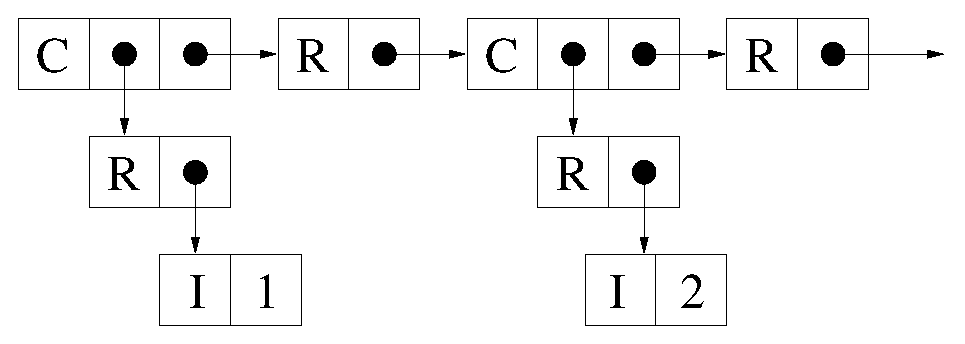
\includegraphics[scale=0.5]{1-Introduction/fig/ref-types/ref-list}
\end{center}

On the other hand, if we define our data types \emph{without} using $\iRef$, then structures of that type can not be updated --- ever. If those structures are provided by a library and a client programmer decides they actually \emph{do} want to perform an update, then it is likely that the only practical solution will be to define their own types and write code that duplicates functionality already present in the original library.

This is exactly the case with SML lists and tuples, which are all immutable. Although some code duplication can be alleviated by using similar module signatures for mutable and immutable objects, the fact that the two have fundamentally different types only serves to encourage it. If only the immutable versions are provided in base libraries, then users are encouraged to use these structures in cases where a mutable one would be more appropriate. This in turn relegates mutable structures to be second class citizens of the language.


\section{Practical limitations of lazy evaluation}
\label{intro:lazy}

The following example from \cite{gustavsson:space-improvement} demonstrates the subtlety of space usage in lazy languages:

\code{
	$\klet$	& $\ixs$	& $= [1..n]$		\\
		& $x$		& $= \ihead \ \ixs$		\\
		& $y$		& $= \ilast \ \ixs$		\\
	$\kin$	& $x + y$
}

We will use GHC as a reference point for the behavior of a real implementation. When compiled with no optimisations, the execution of this program will create a thunk for each let-binding before evaluating the addition~\cite{peyton-jones:g-machine}. If we assume that addition demands its arguments left to right, the thunk for $x$ will be forced first, resulting in the value $1$. This thunk will then be overwritten with its value, which eliminates the contained reference to $\ixs$. The evaluation of $y$ entails the construction and traversal of the list $[1..n]$ until we reach its last element. In a garbage collected implementation this can be done in constant space because $\ilast$ does not hold a reference to a list cell once it has traversed it.

However, if we change the order of arguments to addition the program consumes space proportional to the length of the list:

\code{
	$\klet$	& $\ixs$	& $= [1..n]$		\\
		& $x$		& $= \ihead \ \ixs$		\\
		& $y$		& $= \ilast \ \ixs$		\\
	$\kin$	& $y + x$
}

In this case, the evaluation of $y$ entails the construction of the entire list. The list cannot be garbage collected until the thunk for $\ihead \ xs$ has been forced, because it contains a reference to its first element. This example shows that only slight modifications to a program can result in dramatic differences in space usage.

\subsubsection{All strictness analyses are incomplete}

The run time performance of many lazy programs can be improved by exploiting the \emph{strictness} properties of functions. A function $f$ is \emph{strict} if and only if $f \ \bot \equiv \bot$~\cite{peyton-jones:implementation}. This can arise for three reasons. If $f$ inspects the value of its argument when it evaluates, then it will diverge if its argument does. If $f$ always returns its argument uninspected, then the result will be $\bot$ if the argument is. Finally, $f$ may always diverge, independent of the argument value. If none of these cases apply then function is \emph{non-strict}.

For example, the $\ichoose$ function is strict in its first argument but not the others:

\code{
	$\ichoose \ b \ x \ y = \kif \ b \ \kthen \ x \ \kelse \ y$
}

When this function is applied to its three arguments, it will always require the value of $b$. On the other hand, either $x$ or $y$ may be returned, but not both. A similar example is the $\ifirst$ function which returns just its first argument while discarding the second:

\code{
	$\ifirst \ x \ y = x$
}

As $x$ is passed through to the result, it is strict in this argument. As the function body makes no reference to $y$, it is non-strict in that one. Strictness analysis~\cite{burn:strictness, wadler:projections-strictness, sekar:fast-strictness} is used to recover the strictness properties of functions. A compiler can use this information to convert a call-by-need program into a more call-by-value version without changing its meaning. For an implementation such as GHC, this amounts to identifying the let-bound variables which are passed to strict functions, and evaluating those bindings as soon as they are encountered, instead of building thunks. 

For many lazy programs, especially those performing lots of numeric computation, evaluating strict bindings early can result in substantial performance improvements. Early evaluation saves the allocation and initialisation of thunks, as well the need to update and garbage collect them once their values are demanded.

In practice, a compiler should reduce strict bindings to weak head normal form (whnf)~\cite{peyton-jones:implementation} only. Reduction to whnf eliminates outer redexes while allowing thunks to be present deep within data structures, such as at the tail position of lists. To see why, consider our first example again:

\code{
	$\klet$	& $\ixs$	& $= [1..n]$		\\
		& $x$		& $= \ihead \ \ixs$		\\
		& $y$		& $= \ilast \ \ixs$		\\
	$\kin$	& $x + y$
}

The fact that addition and $\ihead$ are strict in their arguments implies that the $xs$, $x$, and $y$ bindings can be evaluated as soon as they are encountered. If we evaluate $[1..n]$ to whnf we construct just the outer $\iCons$ cell and the program runs in constant space. However, if we were to fully evaluate $[1..n]$ before taking its head, then the program will consume space proportional to this list.

Like all compile time analyses, strictness analysis is necessarily incomplete. This is plainly obvious from our $\ichoose$ example:

\code{
	$\ichoose \ x \ y \ z = \kif \ x \ \kthen \ y \ \kelse \ z$
}

Suppose we write an expression which uses $\ichoose$ to print one of two results:

\code{
	$\iputStr \ (\ichoose \ b \ \iexpOne \ \iexpTwo)$
}

$\iputStr$ is strict in its argument, yet the question of whether it prints $\iexpOne$ or $\iexpTwo$ can only be answered by knowing the value of $b$. In general, the value of $b$ cannot be determined at compile time. Apart from bumping up against the halting problem, this fact is obvious if we consider a situation where $b$ is derived from user input.

In a typical Haskell program, many functions are concerned with processing algebraic data. Such functions are usually written with pattern matching, or with a case-expression that examines the outer constructor of the input value. case-expressions are a generalisation of if-expressions, so we have the same problem as with the $\ichoose$ example above. In general, for a particular function call we can not know what the outer constructor of its argument will be, which defeats strictness analysis in a similar manner.


\subsubsection{Space leaks can be elegantly created with $\imapAccumL$}

In a lazy functional program, a \emph{space leak} is created when unevaluated thunks reference a large amount of data, preventing it from being reclaimed by the garbage collector. This can be counter intuitive at first glance. How can an \emph{unevaluated} expression use more space than its actual result? Consider the expression $(\irange \ 1 \ 100)$ which builds the list $[1..100]$. We would expect a thunk representing the application of $\irange$ to its arguments $1$ and $100$ to use much less space than a fully evaluated list of $100$ elements.

However, consider the case where one of the arguments is a variable instead of an integer value. A thunk which represents the application $(\irange \ 1 \ n)$ contains a reference to the object $n$, and as long as the thunk is live this object cannot be garbage collected. Suppose $n$ is also a thunk, and that it references a large amount of data. While our original list remains unevaluated, this data remains live. It may be that the program's performance would be improved by forcing the list to be fully evaluated as soon as possible. This would allow the garbage collector to reclaim space used by thunks and objects that are no longer referenced. Of course, whether this would work in practice is very application specific. Factors to consider include the size of the resulting list versus the size of the retained data, whether the entire list value will actually be used by the program, whether the live data is also held live by other expressions, cache and main memory sizes, and so on.

Space leaks are especially common in lazy programs which are based around state and state transformers. For these programs, execution is divided into a sequence of steps, with a well-defined state before and after each step. The function $f$ takes the old state, some input $x$ and produces the next state and some output $y$:

\begin{center}
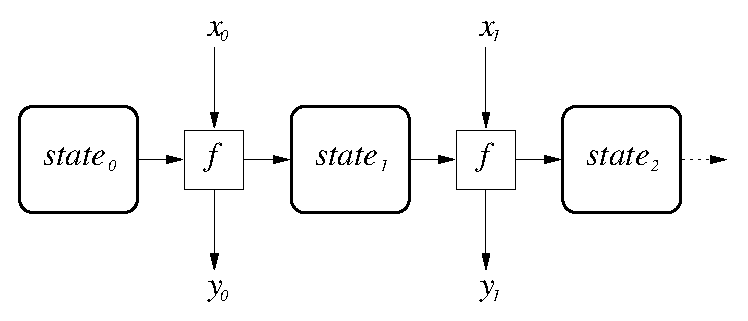
\includegraphics[scale=0.8]{1-Introduction/fig/lazy/space-leak}
\end{center}

\clearpage{}
In Haskell, this pattern of computation is expressed by the function $\imapAccumL$ which has type:
$$\imapAccumL :: (\istate \to x \to (\istate, y)) \to \istate \to [x] \to (\istate, [y])$$

$\imapAccumL$ takes a transition function, an initial state, a list of inputs and produces the final state and the list of outputs. Many programs use a similar pattern of computation, though not all express it with $\imapAccumL$. Consider an interactive program such as a computer game. We could imagine that $\istate$ is a description of the game world, $x$ is the user input, $y$ is a description of the user display, and $f$ is the game logic which computes a new state and display based on the input.

For a computer game, the state could consist of the player's position, surrounding terrain, current enemy positions, remaining ammunition, and so on. A space leak is created when the program fails to demand the entire $y$ value after each step. Suppose that $y$ includes the player's score at each step of the game, but this information is not displayed in real time. Although the score at each step might be expressed by a single integer, as it depends on the current game state at least past of this structure must be kept live until the integer is fully evaluated. If a user plays the game for an hour, with a new state generated 30 times a second, then this can equate to a substantial amount of retained data. Additionally, when the score is a non-trivial function of the current state, reasoning about the \emph{amount} of space wasted becomes intractable.

In Haskell, the only practical way to deal with a complex leak is to write so called $\ideepseq$ functions that manually traverse over an entire structure to ensure it is fully evaluated. Other techniques can help, such as having the garbage collector perform leak avoiding projections~\cite{wadler:fixing-space-leaks}, but to fully cure leaks the programmer must ensure that all structures which \emph{should} be evaluated actually are. Most $\ideepseq$ functions are written to eliminate all redexes in a structure, and are therefore equivalent to the \emph{reduce to normal form} strategy from \cite{trinder:algorithm}. A built-in $\ideepseq$ function was proposed for Haskell', the successor standard to Haskell 98~\cite{haskell-prime:deepseq}, but as of November 2008 it has not been implemented in GHC. 

It is also possible to add strictness annotations to user defined data types. These annotations prevent thunks being created at certain positions in the structure, but cannot be easily be added to library defined types such as $\iMap$ and $\iList$.


\subsubsection{Case study of a space leak}

A state based space leak was encountered while the author was developing a graph coloring register allocator~\cite{chaitin:graph-coloring, smith:graph-coloring} for GHC 6.7. The algorithm is based around a graph where each node represents a program variable. An edge between two nodes represents a constraint that those two variables can not be assigned to the same register. The goal is to assign registers, visualised as colors, to each of the nodes in a way that satisfies the constraints, whilst using only the available set of registers. The algorithm proceeds by extracting a constraint graph from the code undergoing register allocation, and then attempting to color it. If this is not possible with the available colors (registers) then the algorithm modifies the code to store some variables on the stack instead of registers, and tries again. For non-pathological programs this process should converge within three or four iterations.

Graph coloring register allocation is a state based algorithm. The state consists of the current version of the code undergoing allocation, along with the constraint graph. As opposed to the $\imapAccumL$ function, there is no extra per-step input to the state transition function corresponding to the $x$ values in the previous diagram. The output $y$ values correspond to graph profiling information, such as the number of colored versus uncolored nodes remaining after each step.

When the allocator was being developed we were well aware of space leaks and their causes. The intended operation of the algorithm was to build a complete constraint graph, attempt to color it, and if that failed to build a new graph and leave the old one for the garbage collector. We knew that if the program retained any references to the profiling information for old graphs, then this would prevent those graphs from being garbage collected. If this happened we would have a space leak, so we made considerable effort \emph{not} to retain profiling information unless it was explicitly requested. We reasoned that if the user requested profiling information then they would not mind if the allocator ran a little slower due to retained data, as this was not a common operation.

 However, once it was written, an examination of heap space~\cite{sansom:profiling} used by the allocator revealed the following:

\begin{center}
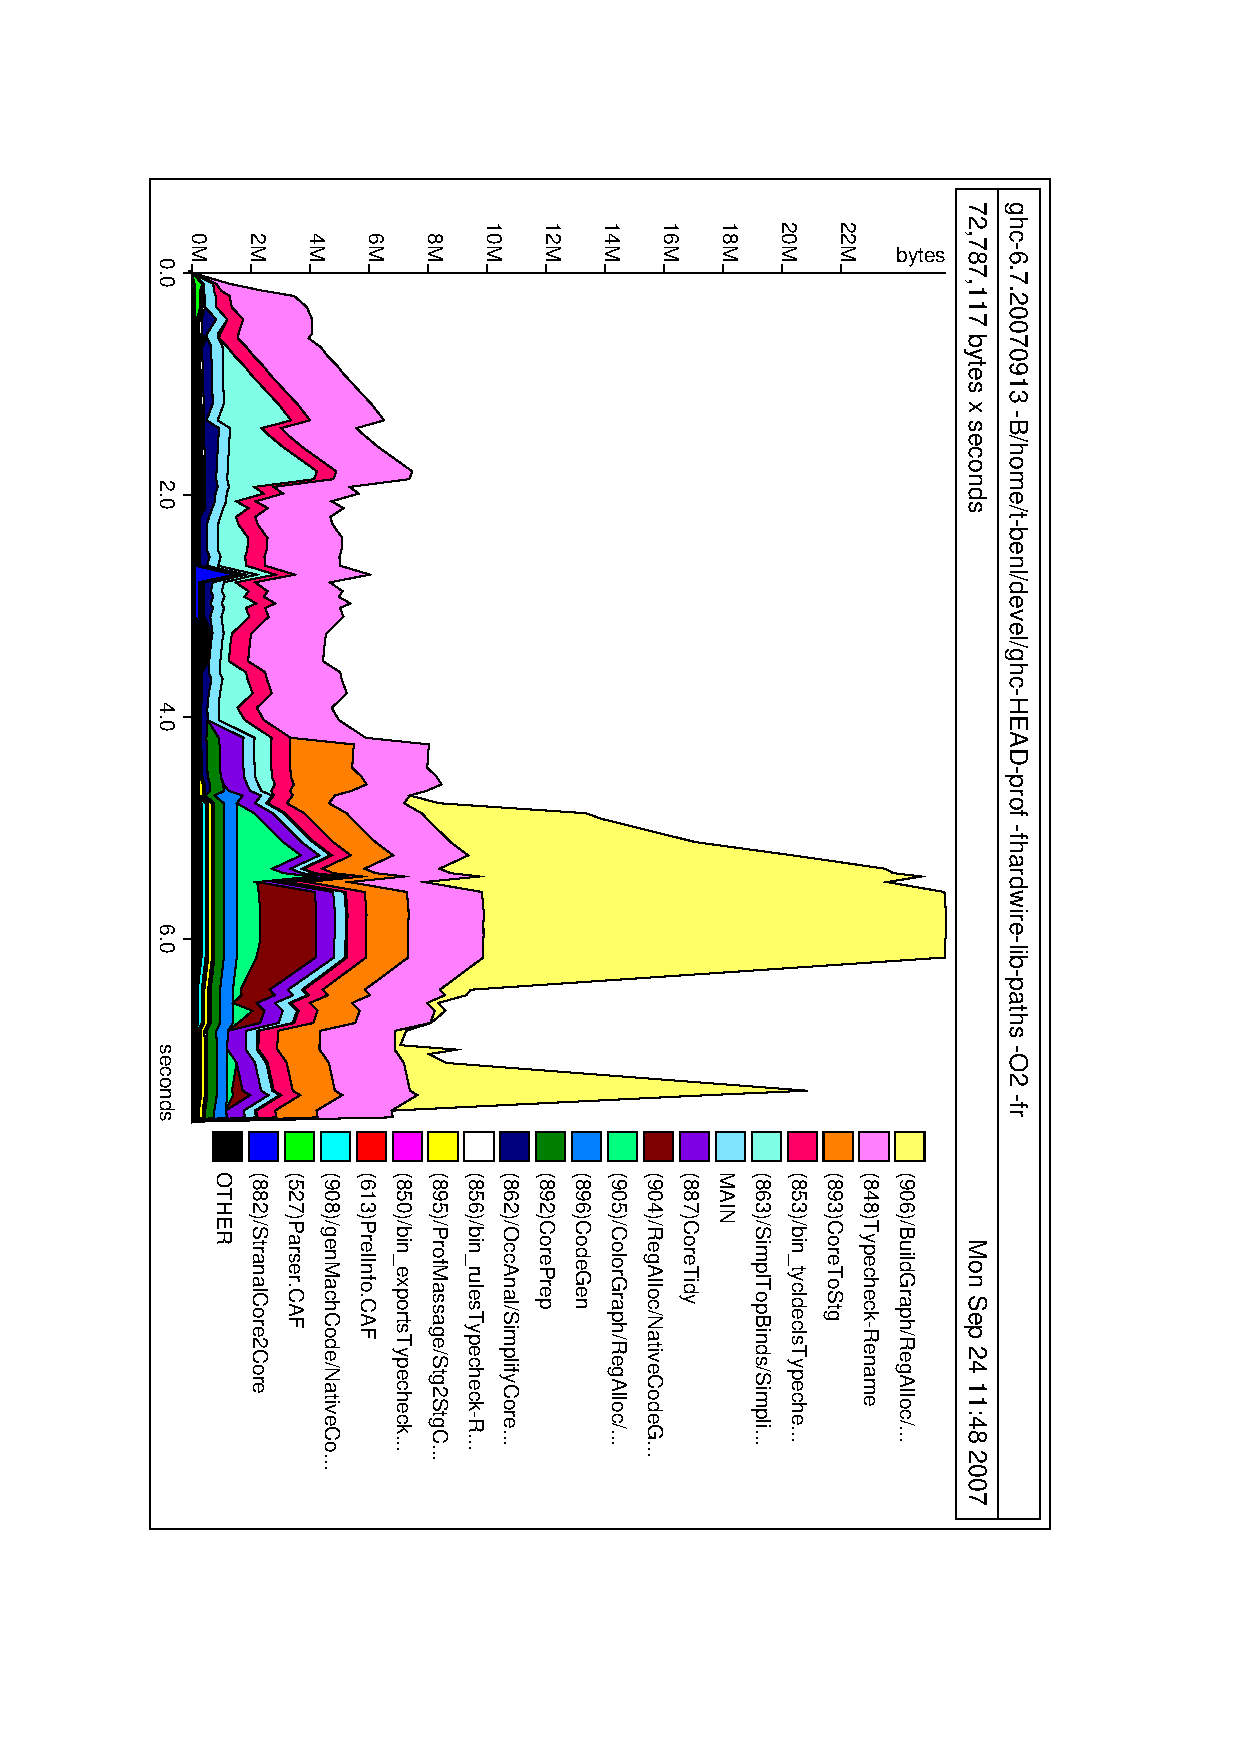
\includegraphics[scale=0.5, angle=90]{1-Introduction/fig/lazy/ghc-sha1-leak.epsi}
\end{center}

The two large spikes in space usage that appear around 6 and 7 seven seconds are directly attributable to the register allocator. This is when performing allocation for the \texttt{SHA1.hs} module from the darcs 1.0.8 source code. Object type profiling revealed that most of the space was taken up by thunks representing function applications.

As to the exact cause of the leak, we are not sure. We could imagine that when the compiler emits a particular compiled machine instruction, this action demands the result of register allocation for that instruction. The registers allocated to a particular instruction depend on what other registers are assigned to surrounding instructions. We could then imagine a section of graph in the final state of the allocator being demanded. This in turn might demand larger sections of graph from previous states, along with parts of the various intermediate versions of assembly code that we tried to find allocation solutions for. 

Good research has been done on formally analysing the space usage of call-by-need programs~\cite{gustavsson:space-improvement, bakewell:space-usage}. However, trying to reason about the exact space behavior of a three thousand line program, compiled with a production compiler that incorporates tens, if not hundreds of individual optimisations is another matter entirely. We plainly admit that our reasoning is little but inspired guess work.

What we do know is that using a $\ideepseq$ function to force the graph to be fully constructed before coloring cured the worst of the problem. This result was obtained through experimentation and frequent consultation with the heap usage profile. The following profile is for the final version:

\begin{center}
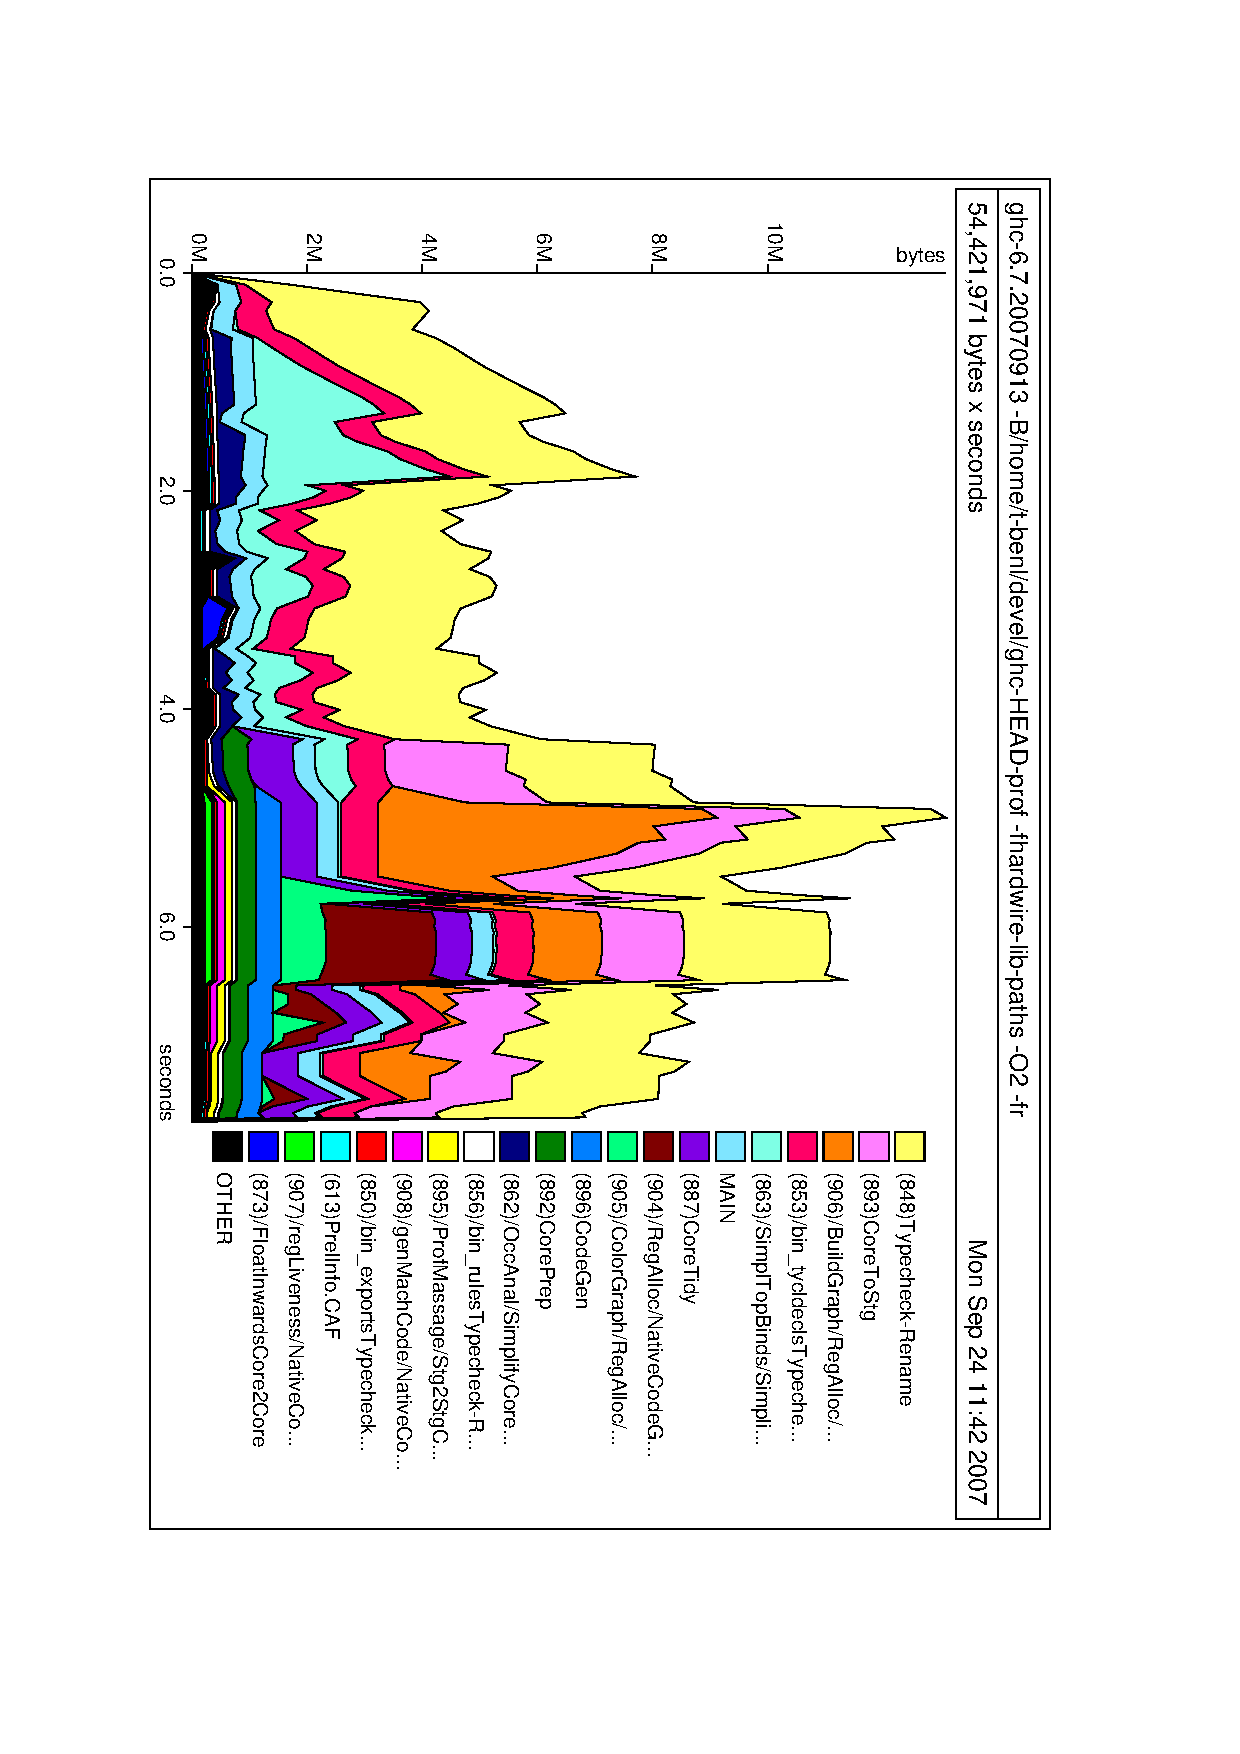
\includegraphics[scale=0.5, angle=90]{1-Introduction/fig/lazy/ghc-sha1-ok.epsi}
\end{center}

In this version the large spikes in space usage have been reduced, resulting in a peak usage around half of the unforced version. We conjecture that the remaining cost attributed to \texttt{(906)/BuildGraph/RegAlloc} is mostly due to the legitimate construction of the graph during allocation, though once again we can not be sure. We deemed the profile acceptable, and moved on to other things.

We glean several points from this experience. Firstly, although a programmer may write what they feel is a state based program, if it is expressed in a lazy language then it may not behave that way at runtime. Secondly, the exact cause of space leaks in large lazy programs can be very hard to reason about. That being said, although the \emph{problem} may be hard to characterise, the solution is well understood. Forcing thunks to values eliminates their contained references and frees up objects for the garbage collector. 

On a philosophical note, we feel there is an immense practical difference between optimisation and control. Having a large number of optimisations in a compiler is all well and good, but if the compiled code \emph{still} doesn't run fast enough then the language (and/or compiler) must provide enough additional control for the programmer to step in and fix the problem. If this is not possible then the programmer will be forced to use a different language, and if that happens more than once then they will be unlikely to choose the same system for their next project.

In this case we were able to fix the problem. However, we do note the irony of writing extra code to manually force the evaluation of expressions that we did not intend to be suspended in the first place. We cannot, off hand, think of a single place in the register allocator code where lazy evaluation was used for a useful purpose. 

We are not suggesting that laziness is never useful, more that it depends on the application. For a selection of programs from the nofib benchmark suite~\cite{partain:nofib}, Harris~\cite{harris:feedback-parallelism} gives the percentage of allocated thunks that were actually evaluated at run-time. In the 20 programs considered, 9 ended up evaluating at least 99\% of their thunks, 14 evaluated at least 90\%, while only one evaluated less than 80\%. 

The fact that a program evaluates almost all of its thunks does not imply it does not make use of laziness. For example, if we use laziness to evaluate the expression $\isum \ [0..100]$ in constant space, then all the thunks in the list will be forced. The application of $\isum$ to a $\iCons$ cell demands the element value as well as the tail of the cell. However, the fact that a program evaluates 99\% of its thunks would suggest that it is not creating lazy lists where the spine is evaluated but the majority of the elements are not. It would also suggest that the program is not using the ``sexier'' lazy structures, such as infinite game trees \cite{hughes:fp-matters}. 





\section{A way forward}

Disciple allows destructive update and lazy evaluation to be present in the same language. We do this while preserving the overall structure of types, and while keeping most of the nice algebraic properties associated with purely functional languages. By preserving the structure of types we hope to avoid the refactoring exercises discussed earlier. We do not rule out support for state monads or $\iRef$ types, rather we desire a system which does not \emph{require} them to write most programs.

We use a type based mutability and effect analysis. The analysis determines which objects in the program might be destructively updated, and which are guaranteed to remain constant. Using this information, the compiler can perform optimisations on the pure parts of the program while leaving expressions with interfering computational effects in their original order. This strategy is similar to that taken by Tolmach~\cite{tolmach:optimizing-ml} though we use a System-F~\cite{reynolds:towards-a-theory-of-type-structure} style core language instead of a monadic one. The core language uses a witness passing mechanism to manage mutability and effect constraints, similar to that used to manage type equality constraints in System-Fc~\cite{sulzmann:system-Fc}. Although the extra mutability and effect information is visible in source types, it can usually be elided by the programmer, and is therefore not an undue burden.

The default evaluation method is call-by-value. This makes it easier to construct an efficient implementation on current hardware, as well as eliminating an important source of space leaks. The programmer may manually suspend function applications when desired, and the runtime system will automatically force them as needed. This is unlike library based implementations of laziness in languages such as O'Caml. These implementations require the use of explicit forcing functions, as well as changing the types of lazy values. 

We also use our analysis to detect when an object is guaranteed \emph{not} to be a thunk. Our implementation of lazy evaluation is likely to be slower than a natively lazy system such as GHC. However, non-lazy code should not suffer a substantial performance penalty compared with other default strict languages such as ML and C.

Our type system uses a type class based mechanism to attach purity, mutability, constancy, laziness and other constraints to data types. This allows functions to be polymorphic in those attributes and not require the overall structure of types to be changed. We also use this mechanism to detect when the combination of laziness and destructive update in the same program might give a result different to the call-by-value case. We flag these as type errors and assert that our language is still purely functional by Sabry's definition~\cite{sabry:purely}. Our language includes support for record types, and we use type directed field projections which permit field names to be in record-local scope. 

We would like for it to be possible \emph{and} practical to write efficient programs in our language. Finally, we would like it to be attractive to people who don't actually care that much about the philosophy of functional programming. We follow Steele and Sussman \cite{steele:lambda-ultimate-imperative}, and Knuth \cite{knuth:structured-programming} in that a language designer's emphasis should be on helping the programmer solve their particular problems. Our aim is not to separate language features into ``good'' and ``bad'', only to offer sharp tools in a hope they will be useful.






